\documentclass[11pt]{article}

% ACL Rolling Review (ARR 2026) template. Change "review" to "final" for camera-ready,
% or to "preprint" for a non-anonymous arXiv version.
\usepackage[review]{acl}

\usepackage{times}
\usepackage{latexsym}
\usepackage[T1]{fontenc}
\usepackage[utf8]{inputenc}
\usepackage{microtype}
\usepackage{inconsolata}
\usepackage{graphicx}
\usepackage{booktabs}
\usepackage{multirow}
\usepackage{amsmath,amssymb}
\usepackage{xcolor}
\usepackage{enumitem}
\usepackage{tikz}
\usepackage{forest}
\usetikzlibrary{arrows.meta,positioning,shapes.misc,decorations.pathreplacing}

% ---- macros ----
\newcommand{\op}[1]{\textsc{#1}}                 % operation names: \op{Predict}
\newcommand{\belief}{\mathbf{b}}
\newcommand{\hist}{H}
\newcommand{\level}[1]{\textbf{#1}}              % credit levels
\newcommand{\todo}[1]{\textcolor{red}{[TODO: #1]}}
\newcommand{\cmark}{\ding{51}}
\newcommand{\xmark}{\ding{55}}
\newcommand{\pmark}{$\circ$}
\usepackage{makecell}
\usepackage{colortbl}
\usepackage[most]{tcolorbox}
\newcommand{\insight}[2]{\begin{tcolorbox}[colback=blue!4,colframe=blue!45!black,boxrule=0.35pt,arc=1.5pt,left=4pt,right=4pt,top=2pt,bottom=2pt,boxsep=0pt,before skip=4pt,after skip=4pt]\footnotesize\textbf{Insight #1.}~#2\end{tcolorbox}}
% Harvey balls
\DeclareRobustCommand{\hbfull}{\tikz[baseline=-0.6ex]{\draw[line width=0.4pt,fill=black] (0,0) circle (0.72ex);}}
\DeclareRobustCommand{\hbhalf}{\tikz[baseline=-0.6ex]{\draw[line width=0.4pt] (0,0) circle (0.72ex); \fill (0,0) -- (90:0.72ex) arc (90:270:0.72ex) -- cycle;}}
\DeclareRobustCommand{\hbnone}{\tikz[baseline=-0.6ex]{\draw[line width=0.4pt] (0,0) circle (0.72ex);}}
\newcommand{\grp}[1]{\rowcolor{gray!12}\multicolumn{6}{@{}l@{}}{\textsc{#1}}\\}
\usepackage{pifont}

\title{From Memory to Belief: A Survey of State Maintenance and Belief Revision in LLM Decision Agents}

\author{Anonymous ARR submission}

\begin{document}
\maketitle

\begin{abstract}
Language-model agents now plan, call tools, and act over many steps, and the failures that dominate reports from such settings are failures of state rather than of reasoning: the agent loses track of what it has learned, keeps acting on evidence that has since been contradicted, or revises what it believes without changing what it does. Memory mechanisms, uncertainty estimation, and post-training with denser rewards each address one part of this problem, but the object that connects them, a persistent, uncertainty-aware belief about a partially observed world, has no survey of its own. This survey takes the belief state as its organising object and traces its development from 2020 to 2026, from context and memory stores through external Bayesian filters and model-written beliefs to learned world models exposed to the policy. We ask one question of every method, \emph{which object receives credit}, the output, the trajectory, the interaction, or the state, and use it to organise three axes: how the belief is represented and whether it commits to testable predictions, how it is revised and where revision fails, and how learning signals reach it. We then align the fragmented belief-level evaluation literature by construct, catalogue 33 benchmarks, and identify the gap the alignment exposes: no published method yet obtains a signed learning signal for a written belief from the agent's own predictions.
\end{abstract}

\section{Introduction}
\label{sec:intro}
\begin{table}[t]
\centering\scriptsize
\setlength{\tabcolsep}{2.2pt}
\renewcommand{\arraystretch}{1.08}
\resizebox{\columnwidth}{!}{%
\begin{tabular}{@{}llc@{\hspace{4pt}}c@{\hspace{4pt}}c@{\hspace{4pt}}c@{}}
\toprule
Survey (venue) & Organising axis & B & R & S & E \\
\midrule
\grp{Memory}
\citet{zhang2024memory} (arXiv) & design, evaluation, use & \hbnone & \hbhalf & \hbnone & \hbnone \\
\citet{hu2025memory} (arXiv) & factual / experiential / working & \hbnone & \hbhalf & \hbnone & \hbhalf \\
\citet{luo2026storage} (ACL F) & storage\,$\to$\,reflection\,$\to$\,experience & \hbnone & \hbhalf & \hbnone & \hbnone \\
\grp{Rewards and credit}
\citet{wu2025rewards} (EMNLP F) & reward model $\times$ stage & \hbnone & \hbnone & \hbnone & \hbnone \\
\citet{zheng2025prm} (ACL) & data $\to$ PRM $\to$ use & \hbnone & \hbnone & \hbnone & \hbnone \\
\citet{zhang2025landscape} (TMLR) & capability $\times$ application & \hbhalf & \hbnone & \hbnone & \hbnone \\
\citet{zhang2026reasoning} (arXiv) & granularity $\times$ method & \hbnone & \hbnone & \hbhalf & \hbnone \\
\grp{Uncertainty}
\citet{xia2025uncertainty} (ACL F) & four estimation avenues & \hbnone & \hbnone & \hbnone & \hbhalf \\
\citet{lin2026uncertainty} (arXiv) & what / how / where & \hbhalf & \hbnone & \hbnone & \hbhalf \\
\grp{Evaluation, horizon, domain}
\citet{yehudai2025survey} (ACL F) & capability $\times$ domain & \hbnone & \hbnone & \hbnone & \hbnone \\
\citet{chen2026horizon} (arXiv) & lifecycle $\times$ horizon carrier & \hbhalf & \hbhalf & \hbnone & \hbnone \\
\citet{xu2026llm} (arXiv) & forecasting architecture & \hbhalf & \hbnone & \hbnone & \hbhalf \\
\citet{dong2025finance} (EMNLP F) & financial function & \hbnone & \hbnone & \hbnone & \hbnone \\
\midrule
\textbf{This survey} & \textbf{credited object} & \hbfull & \hbfull & \hbfull & \hbfull \\
\bottomrule
\end{tabular}}
\caption{Neighbouring surveys and the belief state. \textbf{B}: belief as an object of its own; \textbf{R}: revision and its failure modes; \textbf{S}: learning signals that reach the belief; \textbf{E}: belief-level evaluation. \hbfull\ yes, \hbhalf\ partly, \hbnone\ no.}
\label{tab:surveys}
\end{table}

\begin{figure*}[t]
\centering
\resizebox{\textwidth}{!}{\Forest{
for tree={
  grow'=east, parent anchor=east, child anchor=west, anchor=west,
  draw, rounded corners=2pt, font=\tiny, align=left,
  edge={-, gray!70}, l sep=3.5mm, s sep=0.35mm, fit=band,
  inner xsep=3pt, inner ysep=1.2pt
}
[{\textbf{Belief state} in LLM\\decision agents (\S\ref{sec:formulation})\\\op{Construct} $\cdot$ \op{Test} $\cdot$ \op{Revise}}, fill=blue!10
  [{\S\ref{sec:representation} \textbf{Who maintains}\\\textbf{the belief}}, fill=gray!10
    [{Context as state}, [{CoT \citep{wei2022chain}, ReAct \citep{yao2023react}}]]
    [{External memory}, [{MemGPT \citep{packer2023memgpt}, Generative Agents \citep{park2023generative},\\A-MEM \citep{xu2025amem}, Mem0 \citep{chhikara2025mem0}}]]
    [{Probabilistic memory}, [{BeliefMem \citep{liao2026belief}, D-MEM \citep{song2026d}, Nous \citep{singh2026when}}]]
    [{External Bayesian filter}, [{Belief-State Engine \citep{chattopadhayay2026belief}, Belief at Risk \citep{dixon2026belief},\\BayesEvolve \citep{wu2026bayesevolve}, CAPTURE \citep{hossain2026capture}}]]
    [{Model-written belief}, [{calibrated: DST \citep{lee2021dialogue}, Talker-Reasoner \citep{christakopoulou2024agents},\\Agent-BRACE \citep{singh2026agent}, BOND \citep{cui2026distilling}, BCO \citep{chen2026beliefcalibrated}}] [{testable: Hypothetical Minds \citep{cross2024hypothetical}, CBM \citep{xu2026should}, EvoSCM \citep{zhao2026evoscm}}]]
    [{Learned world model}, [{Dreamer \citep{hafner2023mastering}, RAP \citep{hao2023reasoning}, BB-WM \citep{kumar2026towards};\\written + parametric check: Hybrid-WM \citep{song2026agent}}]]
  ]
  [{\S\ref{sec:revision} \textbf{How revision fails}}, fill=gray!10
    [{Failed stay}, [{BeliefShift \citep{myakala2026beliefshift}, MEDLEY-BENCH \citep{abtahi2026medleybench}}]]
    [{Failed update}, [{STALE \citep{chao2026stale}, DeltaLogic \citep{dhanda2026deltalogic}, DToM-Track \citep{nguyen2026dynamic}}]]
    [{Failed isolation}, [{CBM \citep{xu2026should}, MemOps \citep{hao2026memops}}]]
    [{Failed act}, [{STOCKTAKE \citep{deb2026stocktake}, Werewolf audit \citep{gao2026auditing}}]]
  ]
  [{\S\ref{sec:learning} \textbf{Which object}\\\textbf{receives credit}}, fill=yellow!25
    [{Output}, fill=yellow!10, [{RLHF \citep{ouyang2022training}, DPO \citep{rafailov2023direct}, Self-Refine \citep{madaan2023self}}]]
    [{Trajectory}, fill=yellow!10, [{PRMs \citep{lightman2023lets}, GRPO \citep{shao2024deepseekmath}, LATS \citep{zhou2023language},\\AgentTuning \citep{zeng2023agenttuning}, AgentRefine \citep{fu2025agentrefine}}]]
    [{Interaction}, fill=yellow!10, [{actions: ArCHer \citep{zhou2024archer}, RAGEN \citep{wang2025ragen}, GiGPO \citep{feng2025group}, HiPER \citep{peng2026hiper}}] [{memory operations: MEM1 \citep{zhou2025mem1}, Memento \citep{zhou2025memento}, Memory-R2 \citep{yan2026memoryr2}}]]
    [{State}, fill=yellow!10, [{CBM \citep{xu2026should}, Agent-BRACE \citep{singh2026agent}, BOND \citep{cui2026distilling}}]]
  ]
  [{\S\ref{sec:evidence} \textbf{Evidence acquisition}\\\textbf{conditioned on belief}}, fill=gray!10
    [{BayesEvolve \citep{wu2026bayesevolve}, EvoSCM \citep{zhao2026evoscm}, DenoiseFlow \citep{yan2026denoiseflow}, Bayesian-Agent \citep{wu2026bayesian}}]
  ]
  [{\S\ref{sec:evaluation} \textbf{Belief-level}\\\textbf{evaluation}}, fill=gray!10
    [{Calibration}, [{TC-ECE \citep{lin2026uncertainty}, posterior entropy \citep{dixon2026belief}, FinBench \citep{ghosh2026finbench}}]]
    [{Accuracy and revision}, [{BeliefTrack \citep{xu2026should}, BeliefShift \citep{myakala2026beliefshift}, STALE \citep{chao2026stale}, MemOps \citep{hao2026memops}}]]
    [{Belief--action gap}, [{STOCKTAKE \citep{deb2026stocktake}, Werewolf audit \citep{gao2026auditing}, Agent-ToM \citep{ahmed2026agenttom}}]]
    [{Outcome only}, [{FinBen \citep{xie2025finben}, InvestorBench \citep{li2024investorbench}, HERCULEAN \citep{herculean2026}}]]
  ]
]
}}
\caption{Taxonomy of the survey with representative systems by year. The credited object (yellow) is the axis every method is placed on; Table~\ref{tab:master} in the appendix places every screened system.}
\label{fig:taxonomy}
\end{figure*}


Language-model agents now plan, call tools, retrieve evidence, and act over horizons of hours or months, and the failures reported from these settings are failures of state rather than of reasoning. A model that solves a problem in one pass loses much of its accuracy when the same information arrives over several turns \citep{laban2025lost}; an agent that plans well falls to near-random success once the environment moves while it deliberates \citep{gonzalez2025robotouille}; an agent given only observations wins a fraction of the episodes won by one that reads the simulator's latent state \citep{alaswad2026why}; and in markets, where evidence arrives late and partially, stronger backbones do not reliably produce stronger trading agents \citep{xie2025finben,li2024investorbench}. What these failures share is that the task required the agent to hold something between decisions, a belief about what is true, how certain it is, and what would change it, and the agent never formed it, never tested it, or revised it without acting on the revision.

The field has responded along three lines that rarely cite one another. Memory research moved the state from the reasoning trace \citep{wei2022chain,yao2023react} into external stores that persist, reflect, and abstract experience \citep{park2023generative,shinn2023reflexion,luo2026storage}. Uncertainty research taught models to state confidence \citep{lin2022teaching,kadavath2022language} and extended it from single answers to agent trajectories \citep{lin2026uncertainty}. Post-training moved from rewarding the finished response \citep{ouyang2022training} to rewarding reasoning steps \citep{lightman2023lets,zheng2025prm} and then actions over several turns of interaction \citep{zhou2024archer,zhang2025landscape,zhang2026reasoning}. Each line supervises a different thing, what is stored, how confident the answer is, which action earns reward, and none of them supervises the belief itself.

Explicit beliefs are older than the recent attention suggests: dialogue state tracking wrote one in 2021 \citep{lee2021dialogue}, agents wrote beliefs about tasks, opponents, and markets in 2024 \citep{kim2024qube,cross2024hypothetical,yu2024fincon}, and two 2025 systems learned to overwrite a written state by reinforcement \citep{zhou2025mem1,yu2025memagent}. Until recently the belief was credited, if at all, by the task outcome. In 2026 alone at least twelve systems gave it a learning signal or oracle of its own,\footnote{Belief-State Engine, Belief at Risk and its validation framework, BayesEvolve, CAPTURE, Agent-BRACE, the Bayesian linguistic forecaster, BOND, CBM, BCO, EvoSCM, and the belief-based world model; Section~\ref{sec:representation}.} and benchmarks began to score the belief rather than the outcome it led to \citep{xu2026should,deb2026stocktake,chao2026stale}, with disjoint formalisms and metrics and little mutual citation (timeline in Figure~\ref{fig:timeline}, appendix).

No existing survey takes this object as its own: memory surveys organise by what is stored, reward and credit surveys stop at the action, uncertainty surveys score an output rather than a state, and evaluation surveys report no belief-level metric (Section~\ref{sec:related}, Table~\ref{tab:surveys}). This survey asks one question of every method: \emph{which object receives credit}. Figure~\ref{fig:taxonomy} gives the resulting taxonomy, and Figure~\ref{fig:loop} places the four answers on the observation--belief--action loop: the finished output, the sampled trajectory, the interaction (actions, tool calls, memory operations), or the belief written before the action and tested by evidence returned after it. It cuts across the neighbouring taxonomies rather than replacing them. We cover language-model agents acting over several steps under partial observability, from 2020 to September 2026, collected by a scripted protocol (Appendix~\ref{app:method}). Section~\ref{sec:formulation} grounds the belief state in POMDP belief and belief-revision theory; Sections~\ref{sec:representation}--\ref{sec:evaluation} organise the literature by representation, revision, credited object, evidence acquisition, and evaluation; Section~\ref{sec:discussion} compares the four levels, and Section~\ref{sec:challenges} states the open problems, chief among them that no published method obtains a signed signal for a written belief from the agent's own predictions. Finance is the running example because delayed, partial evidence is its normal condition; the taxonomy is stated without reference to any domain.

\begin{figure}[t]
\centering
\resizebox{0.85\columnwidth}{!}{%
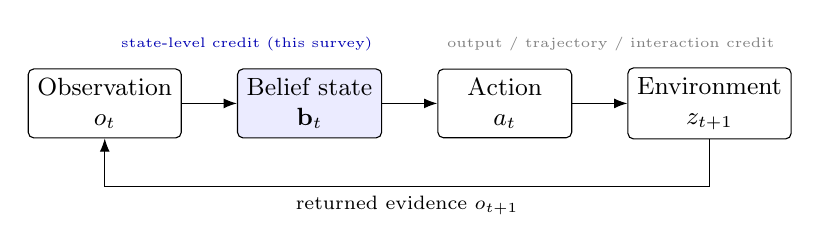
\begin{tikzpicture}[node distance=5mm and 7mm, every node/.style={font=\small}]
\tikzstyle{box}=[draw, rounded corners=2pt, minimum height=7mm, minimum width=17mm, align=center]
\node[box] (obs) {Observation\\$o_t$};
\node[box, right=of obs, fill=blue!8] (bel) {Belief state\\$\belief_t$};
\node[box, right=of bel] (act) {Action\\$a_t$};
\node[box, right=of act] (env) {Environment\\$z_{t+1}$};
\draw[-{Latex}] (obs) -- (bel); \draw[-{Latex}] (bel) -- (act); \draw[-{Latex}] (act) -- (env);
\draw[-{Latex}] (env.south) |- ++(0,-6mm) -| node[pos=0.25, below, font=\scriptsize] {returned evidence $o_{t+1}$} (obs.south);
\node[anchor=south west, font=\tiny, text=gray] at ([yshift=1mm]act.north west) {output / trajectory / interaction credit};
\node[anchor=south east, font=\tiny, text=blue!70!black] at ([yshift=1mm]bel.north east) {state-level credit (this survey)};
\end{tikzpicture}}
\caption{The observation--belief--action loop. Existing post-training credits the action, the trajectory that produced it, or the response text. State-level credit reaches the belief written before the action, using evidence returned after it.}
\label{fig:loop}
\end{figure}

\section{Related Work}
\label{sec:related}

Table~\ref{tab:surveys} places this survey among thirteen neighbouring ones, none of which takes the belief state as its object. Memory surveys \citep{zhang2024memory,hu2025memory,luo2026storage} organise by what is stored and never ask whether a stored item is believed or what evidence would retire it. Reward and credit surveys \citep{wu2025rewards,zheng2025prm,zhang2025landscape,zhang2026reasoning} follow the signal down to tokens, steps, and memory operations and stop at the action. Uncertainty surveys \citep{xia2025uncertainty,lin2026uncertainty} attach a score to an output rather than to a state carried forward. Evaluation, long-horizon, forecasting, and finance surveys \citep{yehudai2025survey,chen2026horizon,xu2026llm,dong2025finance} treat belief as one component among many and report no metric that scores it apart from the outcome.

\section{Problem Formulation}
\label{sec:formulation}

Partially observed decision-making defines the belief as the distribution over hidden variables that is sufficient for acting: with hidden state $z_t$, observation $o_t$, and history $\hist_t$, the belief is $\belief_t = p(z_t \mid \hist_t)$, maintained by a Bayes filter \citep{astrom1965optimal,kaelbling1998planning,thrun2005probabilistic}. Agentic reinforcement learning casts the language-model agent in the same terms, a POMDP whose observable history is the context, with any explicit state kept in a working memory the model itself writes \citep{zhang2025landscape,sumers2023cognitive}. In a ReAct-style agent each turn emits a reasoning segment and then an action \citep{yao2023react}; the reasoning segment is where the state lives, and because the context only grows, the state is carried forward by being rewritten or re-read rather than by an estimator. We write $\belief_t$ for whatever explicit state the span carries before the action $a_t$, and note that a later observation $o_{t+1}$ can evaluate two different things: the action, and the belief that made the action plausible.

Two older literatures say what such a belief must do. Bayesian filtering requires it to predict and to update on the mismatch \citep{thrun2005probabilistic,friston2010free}; belief-revision theory requires that a rational agent can expand its beliefs with a new claim, revise them when a claim is contradicted, and contract them without discarding the rest \citep{alchourron1985logic}. Read together, they give the three operations by which we place every system: \op{Construct}, writing a claim and binding observations to it; \op{Test}, committing to a prediction that a returned observation can falsify; and \op{Revise}, changing the active belief without erasing what was believed. A \emph{memory} stores traces and is judged by recall \citep{luo2026storage}; a \emph{world model} predicts the next observation and is judged by prediction error \citep{li2026bridging}; a \emph{belief} interprets traces as claims about what is true now, with uncertainty, and is judged by calibration and by how fast it is revised when wrong. A reasonable action under a stale belief, the failure that motivates this survey, is invisible to both neighbours.

\section{Belief Representation: Who Maintains the State}
\label{sec:representation}

\begin{table}[t]
\centering\scriptsize
\setlength{\tabcolsep}{3pt}
\renewcommand{\arraystretch}{1.08}
\resizebox{\columnwidth}{!}{%
\begin{tabular}{@{}lccccl@{}}
\toprule
Who maintains the belief & Written & Uncert. & Testable & Auditable & Example \\
\midrule
Context as state & \hbhalf & \hbnone & \hbnone & \hbnone & ReAct \\
External memory & \hbnone & \hbnone & \hbnone & \hbhalf & MemGPT \\
Probabilistic memory & \hbnone & \hbfull & \hbnone & \hbhalf & Nous \\
External Bayesian filter & \hbnone & \hbfull & \hbfull & \hbfull & Belief-State Engine \\
Written, calibrated & \hbfull & \hbfull & \hbnone & \hbhalf & Agent-BRACE, BOND \\
Written, testable & \hbfull & \hbhalf & \hbfull & \hbhalf & CBM, EvoSCM \\
Learned world model & \hbnone & \hbhalf & \hbfull & \hbnone & Dreamer, BB-WM \\
Written + parametric check & \hbfull & \hbfull & \hbfull & \hbhalf & Hybrid-WM \\
\bottomrule
\end{tabular}}
\caption{Representation classes and the properties they trade off. \emph{Written}: the model writes and reads the belief; \emph{Uncert.}: it carries uncertainty; \emph{Testable}: it commits to a falsifiable prediction; \emph{Auditable}: it can be validated against a closed-form oracle. \hbfull\ yes, \hbhalf\ partly, \hbnone\ no.}
\label{tab:reprprops}
\end{table}


Where does the belief live, who writes it, and can it be wrong in a way that later evidence can show? We order representations by \emph{who maintains the belief}, from no one to an explicit estimator, and by whether the belief is \emph{testable}, that is, commits to a prediction that a returned observation can falsify. Table~\ref{tab:reprprops} summarises the classes; Figure~\ref{fig:repr} and Table~\ref{tab:master} in the appendix place every system on both axes.

\subsection{Context and Memory}
\label{sec:repr:memory}

The most common design has no representation at all: the reasoning trace is the state \citep{wei2022chain,yao2023react}, the belief implicit and its uncertainty unstated. In a text game, agents that read the simulator's latent state win about 79\% of episodes against 11\% for agents that read only observations \citep{alaswad2026why}, and on STALE the best model resolves old-versus-new conflicts in 55\% of cases \citep{chao2026stale}, and programmatic state abstraction alone helps substantially \citep{bogdanov2026context,he2026ycbench}.

Memory-augmented agents moved the state into a store retrieved into context \citep{packer2023memgpt,park2023generative,zhong2024memorybank,xu2025amem}, the evolution that \citet{luo2026storage} survey. Two limits matter for belief: the stored unit is a trace rather than a claim with a probability, and an update is an operation on the store rather than on a hypothesis, so answer accuracy hides failures in the update and forget operations themselves \citep{hao2026memops}. Structured stores narrow the first limit with schemas, graphs, or bitemporal transitions \citep{xu2026nesyfs,luo2026graph,liu2026made,xu2026governed,ning2026evoharness}; probabilistic stores narrow the second by attaching a number to each claim \citep{liao2026belief,song2026d,yang2026belief}. Even closed-form Bayesian updates per stored claim barely beat last-write-wins on LoCoMo \citep{singh2026when,srivastava2026causal}.

\subsection{External Bayesian Filters}
\label{sec:repr:filter}

A different line takes the belief out of the model. The model maps evidence to a likelihood over a fixed set of latent regimes, hypotheses, or user states, and an explicit filter maintains the posterior, whose entropy and drift can then be reported as model risk \citep{chattopadhayay2026belief,dixon2026belief,dixon2026model,dixon2026adaptive,wu2026bayesevolve,hossain2026capture,soru2026semantic}. These are the only beliefs in the survey validated against a closed-form oracle, and they are auditable by construction. The price is a hypothesis space fixed in advance: the filter cannot introduce a factor it was not given.

\subsection{Model-Written Beliefs}
\label{sec:repr:written}

The third line keeps the belief in context but gives it structure the model writes and reads. Dialogue state tracking wrote a slot-value belief in 2021 \citep{lee2021dialogue}, verbalised confidence attached a probability to an answer \citep{lin2022teaching,kadavath2022language}, 2024 agents wrote beliefs about tasks, opponents, and markets \citep{kim2024qube,christakopoulou2024agents,cross2024hypothetical,yu2024fincon}, and in 2025 MEM1 and MemAgent learned to overwrite a fixed written state each turn \citep{zhou2025mem1,yu2025memagent}. The newest systems add uncertainty and verification to the written object, from certainty tags and Bayesian-teacher posteriors to symbolic verification and populations of causal models \citep{singh2026agent,murphy2026agentic,cui2026distilling,xu2026should,chen2026beliefcalibrated,seo2026assumptions,giovannelli2026chal,zhao2026evoscm}.

Testability separates them, and we define it operationally: a written belief is testable if it contains a statement about a future observation with a horizon, so that the returned observation yields a signed error for that statement. By this definition most written beliefs are calibrated but not testable: they state confidence or revise the belief but never name the observation that would falsify it. Hypothetical Minds, CBM, and EvoSCM do, and Section~\ref{sec:learning} turns on this distinction.

\subsection{Learned World Models}
\label{sec:repr:wm}

The fourth line learns the dynamics and exposes the resulting belief to the policy: recurrent latent states \citep{ha2018world,hafner2019learning,hafner2023mastering}, the language model as its own world model for tree search \citep{hao2023reasoning,zhao2023large,zhou2023language}, LLM-proposed POMDPs refined to a belief-based likelihood \citep{six2026learning}, and a world-model belief the policy can query \citep{kumar2026towards,li2026bridging,bagaria2026recursive}. World-model beliefs are testable by construction but, unless written back, cannot be reasoned about in language. Two 2026 systems close that gap by using the learned model as a check on a written belief rather than a replacement: a parametric consistency gate that cuts the hallucinated-state rate from 0.176 to 0.035 \citep{song2026agent}, and semantic rules distilled from prediction--observation mismatches \citep{zhang2026selfevolvingx}. 

\insight{1}{\textbf{Structure is not testability.} Memory design has made the belief steadily more structured without making it falsifiable, and the representations that can be falsified, filters and world models, cannot be reasoned about in language. The belief the field needs is written and testable at once; no peer-reviewed system has one yet.}

\section{Belief Revision and Its Failure Modes}
\label{sec:revision}

\begin{figure}[t]
\centering
\resizebox{\columnwidth}{!}{%
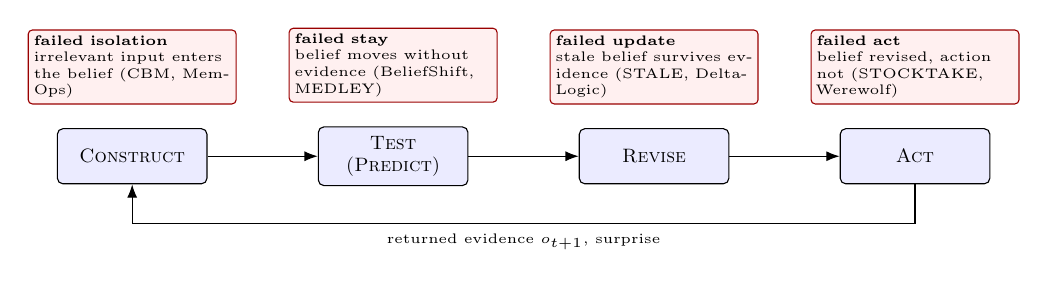
\begin{tikzpicture}[font=\scriptsize,
  op/.style={draw, rounded corners=2pt, fill=blue!8, minimum width=19mm, minimum height=7mm, align=center, font=\scriptsize\scshape},
  fail/.style={draw=red!60!black, fill=red!6, rounded corners=1.5pt, align=left, font=\tiny, inner sep=2pt, text width=25mm}]
\node[op] (c) {Construct};
\node[op, right=14mm of c] (t) {Test\\(\op{Predict})};
\node[op, right=14mm of t] (rv) {Revise};
\node[op, right=14mm of rv] (a) {Act};
\draw[-{Latex}] (c) -- (t); \draw[-{Latex}] (t) -- (rv); \draw[-{Latex}] (rv) -- (a);
\draw[-{Latex}] (a.south) |- ++(0,-5mm) -| node[pos=0.25, below, font=\tiny] {returned evidence $o_{t+1}$, surprise} (c.south);
\node[fail, above=3mm of c] (f3) {\textbf{failed isolation}\\ irrelevant input enters the belief (CBM, MemOps)};
\node[fail, above=3mm of t] (f1) {\textbf{failed stay}\\ belief moves without evidence (BeliefShift, MEDLEY)};
\node[fail, above=3mm of rv] (f2) {\textbf{failed update}\\ stale belief survives evidence (STALE, DeltaLogic)};
\node[fail, above=3mm of a] (f4) {\textbf{failed act}\\ belief revised, action not (STOCKTAKE, Werewolf)};
\end{tikzpicture}}
\caption{Where the four failure modes of Section~\ref{sec:revision} occur on the construct--test--revise--act cycle. Only a testable belief lets returned evidence be routed to the operation that failed rather than to the action.}
\label{fig:failures}
\end{figure}

\begin{table}[t]
\centering\scriptsize
\setlength{\tabcolsep}{3pt}
\renewcommand{\arraystretch}{1.08}
\resizebox{\columnwidth}{!}{%
\begin{tabular}{@{}lp{2.05cm}p{1.75cm}p{1.9cm}@{}}
\toprule
Failure mode & Definition & Measured by & Headline result \\
\midrule
Failed stay & belief moves without evidence & BeliefShift, MEDLEY-BENCH & consensus sensitivity from near 0 to large across 35 models \\
Failed update & belief survives contradicting evidence & DeltaLogic, DToM-Track, STALE & 66.7\% on a conclusion, 46.7\% on whether an edit changes it \\
Failed isolation & irrelevant input enters the belief & BeliefTrack, MemOps & belief-state reward cuts failures by 71\% \\
Failed act & belief revised, action unchanged & STOCKTAKE, Werewolf audit & 34--43\% of correctly diagnosed weeks end in the wrong action \\
\bottomrule
\end{tabular}}
\caption{Four failure modes of belief revision, the benchmarks that isolate each, and their headline results \citep{myakala2026beliefshift,abtahi2026medleybench,dhanda2026deltalogic,nguyen2026dynamic,chao2026stale,xu2026should,hao2026memops,deb2026stocktake,gao2026auditing}.}
\label{tab:failures}
\end{table}


Bayesian filtering and active inference agree on how a belief should change: it predicts, evidence arrives, and the mismatch drives the update \citep{friston2010free,friston2017active}; factor graphs then assign the error to the factors that produced the prediction \citep{kschischang2001factor,loeliger2004introduction}. The language-model literature imported the vocabulary but rarely the routing: feedback is appended to the context or folded into self-critique loops that revise an output, a plan, or a trajectory \citep{huang2022inner,madaan2023self,chen2023teaching,kim2023language,wang2023describe}.

\subsection{Four Failure Modes}
\label{sec:rev:modes}

Contextual Belief Management names three ways a belief can fail on new input, a \emph{failed stay} in which the belief moves without evidence, a \emph{failed update} in which it survives evidence against it, and a \emph{failed isolation} in which irrelevant input contaminates it \citep{xu2026should}. Three independent studies document a fourth, the \emph{failed act}, in which the belief is revised but the action is not, so that a belief-level oracle finds the diagnosis right while the action stays wrong \citep{deb2026stocktake,gao2026auditing}. Table~\ref{tab:failures} lists the benchmark that isolates each mode; their placement on the construct--test--revise--act cycle (Figure~\ref{fig:failures}) is ours, and each names the operation whose signal should receive the error.

\subsection{Mechanisms of Revision}
\label{sec:rev:mech}

Failed update is now a benchmark topic in its own right \citep{chao2026stale,sun2026memory,nakayashiki2026stale,yang2026groupmembench}; in finance it is a stale factor, visible as drift in the agent's planning embeddings before the trading loss appears \citep{xue2026representation}. The mechanisms that respond fall into three families by what triggers them. The first is triggered by \emph{contradiction} among stored claims and resolves it with an operator algebra, first-class update and forget operations, or supersession contracts that keep the superseded claim visible \citep{wang2026toki,hao2026memops,xu2026governed}. The second is triggered \emph{before commitment}, by self-audit, a parametric veto, semantic entropy, or resampling \citep{yuan2026verify,song2026agent,yan2026denoiseflow,wang2026t2po}; these see no future observation and so cannot catch a belief that is consistent and wrong. The third is triggered by \emph{surprise}: reward-prediction error routes writes to a fast or a slow path \citep{song2026d}, and prediction--observation mismatches become semantic rules \citep{zhang2026selfevolvingx}.

Routing the error to the claim that produced the prediction, the factor-graph step with which this section opened, is what none of the surveyed systems implements in the model's own context.

\insight{2}{\textbf{Revision is triggered, not routed.} Contradiction, self-audit, and surprise decide \emph{when} a belief changes; none decides \emph{which claim} the error belongs to. Until the error is routed to the claim that made the prediction, agents will keep repairing memories while beliefs stay wrong, and failed act will remain the unmeasured mode.}

\section{Learning Signals by Credited Object}
\label{sec:learning}

\begin{figure}[t]
\centering
\resizebox{\columnwidth}{!}{%
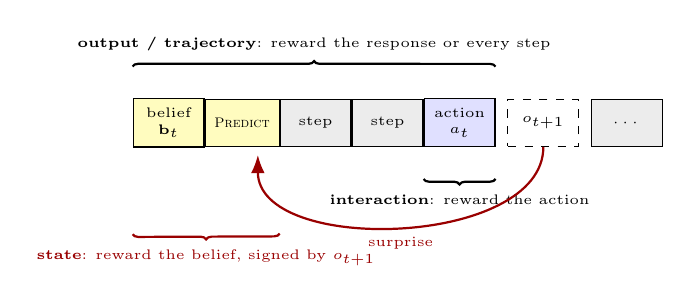
\begin{tikzpicture}[font=\scriptsize,
  tok/.style={draw, minimum width=9mm, minimum height=6mm, align=center, font=\tiny},
  lvl/.style={font=\tiny, anchor=east}]
% one span of a trajectory: b_t (written belief) then a_t (action), then o_{t+1}
\node[tok, fill=yellow!25] (b1) at (0,0) {belief\\$\belief_t$};
\node[tok, fill=yellow!25, right=0mm of b1] (b2) {\op{Predict}};
\node[tok, fill=gray!15, right=0mm of b2] (r1) {step};
\node[tok, fill=gray!15, right=0mm of r1] (r2) {step};
\node[tok, fill=blue!12, right=0mm of r2] (a1) {action\\$a_t$};
\node[tok, dashed, right=1.5mm of a1] (o1) {$o_{t+1}$};
\node[tok, fill=gray!15, right=1.5mm of o1] (nx) {$\cdots$};
% credit brackets
\draw[decorate, decoration={brace, amplitude=2pt}, thick] ([yshift=4mm]b1.north west) -- ([yshift=4mm]a1.north east) node[midway, above=2pt, font=\tiny] {\textbf{output / trajectory}: reward the response or every step};
\draw[decorate, decoration={brace, amplitude=2pt, mirror}, thick] ([yshift=-4mm]a1.south west) -- ([yshift=-4mm]a1.south east) node[midway, below=2pt, font=\tiny] {\textbf{interaction}: reward the action};
\draw[decorate, decoration={brace, amplitude=2pt, mirror}, thick, red!60!black] ([yshift=-11mm]b1.south west) -- ([yshift=-11mm]b2.south east) node[midway, below=2pt, font=\tiny, text=red!60!black] {\textbf{state}: reward the belief, signed by $o_{t+1}$};
\draw[-{Latex}, red!60!black, thick] (o1.south) to[out=-90, in=-90, looseness=0.9] node[pos=0.5, below, font=\tiny, text=red!60!black] {surprise} ([xshift=2mm,yshift=-1mm]b2.south);
\end{tikzpicture}}
\caption{The credited object on one span of a trajectory. Output- and trajectory-level credit reaches text generated from the context; interaction-level credit reaches the action; state-level credit reaches the written belief, and its sign comes from the observation returned after the action.}
\label{fig:credit}
\end{figure}

\begin{table}[t]
\centering\scriptsize
\setlength{\tabcolsep}{3pt}
\renewcommand{\arraystretch}{1.08}
\resizebox{\columnwidth}{!}{%
\begin{tabular}{@{}llll@{}}
\toprule
Level & Credited object & Signed by $o_{t+1}$? & Representative \\
\midrule
Output & finished response & no & RLHF, DPO \\
Trajectory & sampled steps & no & PRMs, GRPO, LATS \\
Interaction & actions, tool calls & no (task reward) & ArCHer, RAGEN, HiPER \\
Interaction & memory operations & no (operation reward) & MEM1, Memento, Memory-R2 \\
State & written belief & closed-world oracle & CBM \\
State & claim + certainty & calibration target & Agent-BRACE \\
State & posterior tag & Bayesian teacher & BOND \\
State & written belief & \emph{own prediction} & (none published) \\
\bottomrule
\end{tabular}}
\caption{Learning signals by credited object and where the sign of the signal comes from (Section~\ref{sec:learning}); the full version with feedback source, granularity, and evidence level is Table~\ref{tab:learning} in the appendix.}
\label{tab:learningmain}
\end{table}


Existing surveys organise post-training by where the reward comes from, where the trajectories come from, and how dense the signal is \citep{wu2025rewards,zhang2026reasoning,zheng2025prm}. We hold those fixed and vary one thing, the object that receives the gradient (Figure~\ref{fig:credit}, Table~\ref{tab:learningmain}). The criterion is operational: a method is at the \emph{state level} if the quantity that receives a gradient is a claim about the environment and its sign depends on an observation returned after the action. A method that rewards a memory write regardless of whether the written claim was true is at the interaction level, however dense its credit.

\subsection{Output and Trajectory}
\label{sec:learn:traj}

Supervised fine-tuning and preference optimisation credit the completed response \citep{ouyang2022training,wei2022finetuned,rafailov2023direct}, and self-consistency and self-improvement select the responses to train on \citep{wang2022self,huang2022large}. Trajectory-level credit began by imitating and searching over agent trajectories \citep{chen2023fireact,zeng2023agenttuning,xi2024agentgym,zhou2023language,putta2024agent,fu2025agentrefine}, then credited sampled steps directly through PPO, GRPO, and process reward models \citep{schulman2017proximal,shao2024deepseekmath,lightman2023lets,zheng2025prm,zhang2026selfevolving,tan2026hindsight}.

\subsection{Interaction}
\label{sec:learn:inter}

Agentic reinforcement learning credits actions over several turns \citep{zhou2024archer,qi2024webrl,wang2025ragen,chen2025reinforcement,zhou2025sweetrl,feng2025group,dong2025agentic}, and the open question is how to make that credit denser without making it wrong, by hierarchical advantages, counterfactual estimators over shared states, potential-based shaping, or verifier-structured credit \citep{peng2026hiper,wang2026capo,diao2026hipif,wang2026groupgraph,ren2026iapo,liao2026tcpo,he2026turns,liu2026pica,xie2026tips,zheng2026pgpo,zhang2026mica,li2026vict,wang2026teach,guo2026hidifftir,qi2026stapo,zhao2026aem,lin2026skillc}; denser is not free \citep{modecrua2026multiturn,pu2026explore}. The nearest this level comes to the state is a group that credits the write to a memory, from a rewritten case bank to an RL-trained overwrite of a fixed written state \citep{zhou2025memento,zhou2025mem1,yu2025memagent,yan2026memoryr2,wang2026tamtrl,ning2026evoharness,wang2026slearl,hu2026collaborative}. By the criterion above these remain interaction-level: they credit the \emph{operation}, so a well-executed update to a wrong claim is still rewarded.

\subsection{State}
\label{sec:learn:state}

Three published methods meet the criterion. CBM trains with belief-state rewards from symbolic verification and cuts belief-management failures by about 71\% \citep{xu2026should}. Agent-BRACE trains belief model and policy jointly with verbalised certainty as the belief's output \citep{singh2026agent}. BOND distils a Bayesian teacher's posterior into an 8B student whose Brier score beats a 70B prompted baseline \citep{cui2026distilling}.

\insight{3}{\textbf{Credit has been getting denser, not deeper.} Agentic reinforcement learning has refined which action to prefer; no method changed what the action is conditioned on. The two axes are orthogonal, and the first system to combine them will need a sign for its belief that the environment, not an oracle, supplies.}

\section{Belief-Guided Evidence Acquisition}
\label{sec:evidence}

\begin{table}[t]
\centering\scriptsize
\setlength{\tabcolsep}{3pt}
\renewcommand{\arraystretch}{1.08}
\resizebox{\columnwidth}{!}{%
\begin{tabular}{@{}p{2.2cm}p{2.9cm}p{2.3cm}@{}}
\toprule
Acquisition conditioned on & Systems & Belief object \\
\midrule
fixed heuristic & agentic RAG \citep{gao2024rag} & none \\
task-level POMDP & CGDP \citep{kausik2026context}, MedExAgent \citep{gao2026medexagent} & searcher, patient state \\
uncertainty of an explicit belief & BayesEvolve \citep{wu2026bayesevolve}, EvoSCM \citep{zhao2026evoscm}, DenoiseFlow \citep{yan2026denoiseflow} & hypothesis posterior, causal population, step entropy \\
belief over own resources & Bayesian-Agent \citep{wu2026bayesian}, REDEREF \citep{hosseini2026trainingfree}, CMI \citep{srivastava2026causal} & skill, delegate, memory reliability \\
information gain as reward & PiCA \citep{liu2026pica}, TIPS \citep{xie2026tips} & implicit \\
written testable belief & \emph{none found} & --- \\
\bottomrule
\end{tabular}}
\caption{Evidence-acquisition decisions by what they are conditioned on.}
\label{tab:evidence}
\end{table}

A testable belief tells the agent what evidence would change it, which turns retrieval, tool use, and routing from fixed pipeline stages into decisions (Table~\ref{tab:evidence}). Agentic search \citep{kausik2026context} and clinical diagnosis \citep{gao2026medexagent} have been framed as POMDPs whose actions include what to observe next, and two finance simulators show why it matters: failing agents spend 62\% of their observation budget re-reading internal state, and failures trace to incomplete acquisition rather than to reasoning \citep{han2026can,zhang2026retailbenchx}.

The methods that condition acquisition on a belief differ in what the belief is over (Table~\ref{tab:evidence}). Agentic retrieval first let the model decide when to retrieve \citep{gao2024rag}; recent systems condition that decision on measured uncertainty about the task \citep{wu2026bayesevolve,zhao2026evoscm,xu2026nesyfs,yan2026denoiseflow}, make information gain the training signal itself \citep{liu2026pica,xie2026tips}, or keep a belief over the agent's own skills, delegates, or memories \citep{wu2026bayesian,hosseini2026trainingfree,srivastava2026causal}. Financial evidence adds a constraint, since much of it cannot leave its silo; knowledge harnesses and federated adaptation are the compliance-aware forms of integration \citep{borjigin2026absorbing,concordia2026}. 

\insight{4}{\textbf{Acquisition is a belief problem.} Agents lose by re-reading what they know rather than seeking what would change it. A testable belief names that evidence, so evidence acquisition will move from a fixed retrieval stage to a consequence of the belief.}

\section{Evaluating Belief Apart from Outcome}
\label{sec:evaluation}

\begin{figure}[t]
\centering
\resizebox{\columnwidth}{!}{%
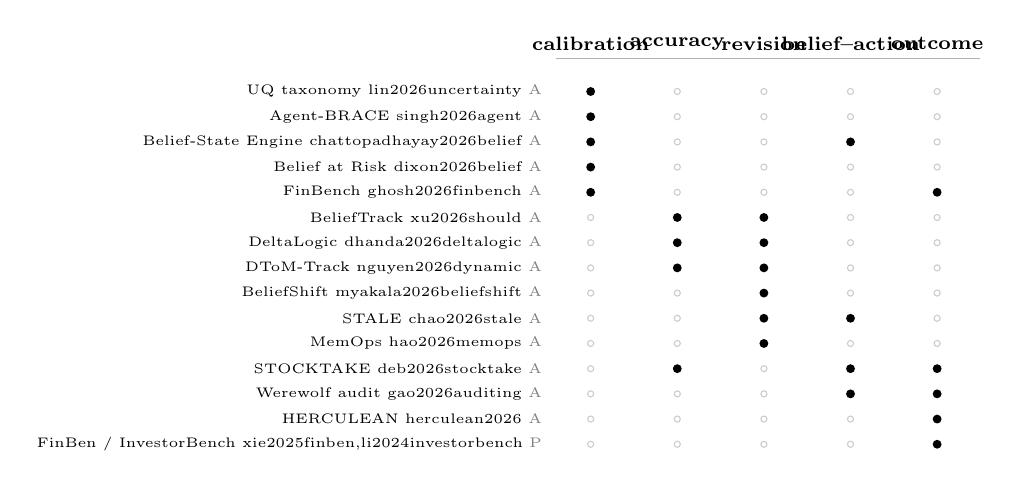
\begin{tikzpicture}[font=\scriptsize, x=11mm, y=3.2mm]
\foreach \c/\x in {calibration/1, accuracy/2, revision/3, belief--action/4, outcome/5} \node[align=center, font=\scriptsize\bfseries, rotate=0] at (\x,0.9) {\c};
\foreach \name/\ev/\y/\dots in {
  {UQ taxonomy \citep{lin2026uncertainty}}/A/-1/{1},
  {Agent-BRACE \citep{singh2026agent}}/A/-2/{1},
  {Belief-State Engine \citep{chattopadhayay2026belief}}/A/-3/{1,4},
  {Belief at Risk \citep{dixon2026belief}}/A/-4/{1},
  {FinBench \citep{ghosh2026finbench}}/A/-5/{1,5},
  {BeliefTrack \citep{xu2026should}}/A/-6/{2,3},
  {DeltaLogic \citep{dhanda2026deltalogic}}/A/-7/{2,3},
  {DToM-Track \citep{nguyen2026dynamic}}/A/-8/{2,3},
  {BeliefShift \citep{myakala2026beliefshift}}/A/-9/{3},
  {STALE \citep{chao2026stale}}/A/-10/{3,4},
  {MemOps \citep{hao2026memops}}/A/-11/{3},
  {STOCKTAKE \citep{deb2026stocktake}}/A/-12/{2,4,5},
  {Werewolf audit \citep{gao2026auditing}}/A/-13/{4,5},
  {HERCULEAN \citep{herculean2026}}/A/-14/{5},
  {FinBen / InvestorBench \citep{xie2025finben,li2024investorbench}}/P/-15/{5}}
 {\node[anchor=east, font=\tiny] at (0.55,\y) {\name~{\color{gray}\ev}};
  \foreach \x in {1,...,5} \draw[gray!40] (\x,\y) circle (1.1pt);
  \foreach \x in \dots \fill (\x,\y) circle (1.6pt);}
\draw[gray!60] (0.6,0.3) -- (5.5,0.3);
\end{tikzpicture}}
\caption{Which belief-level construct each evaluation paper reports. Filled dots mark a reported metric. \textsf{P} = peer-reviewed venue, \textsf{A} = arXiv preprint at the time of writing. No two papers report the same metric for the same construct, which is the fragmentation this section addresses.}
\label{fig:metrics}
\end{figure}


A realised trade or a correct answer can follow from a correct belief, from a wrong belief that did not matter, or from a belief revised too late, and outcome metrics cannot separate the three; this is why stronger backbones do not yield stronger trading agents and the benchmarks cannot say why \citep{xie2025finben,li2024investorbench}. Earlier agent benchmarks score task success or recall \citep{shridhar2020alfworld,liu2023agentbench,maharana2024evaluating,yao2024taubench}; recent work responded with belief-level metrics, each paper defining its own. Figure~\ref{fig:metrics} aligns them by construct, and Table~\ref{tab:benchmarks} in the appendix catalogues 33 benchmarks by whether the evaluator can observe the latent state.

\subsection{Constructs}
\label{sec:eval:constructs}

\emph{Calibration over a trajectory} has the most statistics and the least comparability: checkpoint calibration error, episode-level calibration, posterior entropy, and proper scoring rules on time-gated forecasts express one construct in four ways, none computed on another paper's system \citep{lin2026uncertainty,singh2026agent,chattopadhayay2026belief,dixon2026belief,ghosh2026finbench}. \emph{Belief accuracy and revision} are measured against a known answer in a closed world, after a minimal premise edit, and across recall, inference, and change detection \citep{xu2026should,dhanda2026deltalogic,nguyen2026dynamic}, and against human annotation \citep{myakala2026beliefshift,chao2026stale,hao2026memops,yang2026groupmembench} and, for beliefs about other agents, by theory-of-mind benchmarks \citep{bawatneh2026omnitom,wang2026mindgames}. The \emph{belief--action gap} is the youngest construct: STOCKTAKE scores the agent against an exact Bayes filter on the same observations \citep{deb2026stocktake}, the Werewolf audit reports action--belief consistency \citep{gao2026auditing}, and Agent-ToM monitors an agent's beliefs from its trajectory \citep{ahmed2026agenttom}.

\subsection{Where the Latent State Comes From}
\label{sec:eval:latent}

Every construct beyond calibration needs a latent state to compare against. Controlled environments provide it \citep{deb2026stocktake,xu2026should,alaswad2026why}; long-horizon simulators know it but report belief only through proxies \citep{he2026ycbench,zhang2026retailbenchx,han2026can}; historical replay provides neither, so workflow benchmarks can report a belief failure only at the outcome level \citep{herculean2026}. 

\insight{5}{\textbf{Belief cannot be scored by outcome.} Five constructs, fifteen metrics, no cross-paper comparison; only the fair oracle scores belief and action on the same episodes. Progress on belief will be measurable only where the latent state is known, so controlled environments, not replay, are where the next results should come from.}

\section{Discussion}
\label{sec:discussion}

\begin{table}[t]
\centering\scriptsize
\setlength{\tabcolsep}{3pt}
\renewcommand{\arraystretch}{1.08}
\resizebox{\columnwidth}{!}{%
\begin{tabular}{@{}llccccc@{}}
\toprule
Level & Sign of the signal from & Env. & No oracle & Belief & Act gap & Maturity \\
\midrule
Output & humans, verifiers & \hbnone & \hbhalf & \hbnone & \hbnone & \hbfull \\
Trajectory & verifier, PRM & \hbhalf & \hbhalf & \hbnone & \hbnone & \hbfull \\
Interaction (actions) & task reward & \hbfull & \hbfull & \hbnone & \hbnone & \hbfull \\
Interaction (memory ops) & task reward, teacher & \hbfull & \hbhalf & \hbhalf & \hbnone & \hbhalf \\
State (oracle or teacher) & closed world, teacher, target & \hbnone & \hbnone & \hbfull & \hbfull & \hbhalf \\
State (own prediction) & returned observation & \hbfull & \hbfull & \hbfull & \hbfull & \hbnone \\
\bottomrule
\end{tabular}}
\caption{The four credit levels compared. \emph{Env.}: the sign of the signal comes from the environment; \emph{No oracle}: no external source of truth is needed; \emph{Belief}: the written belief receives the gradient; \emph{Act gap}: belief error and action error are separated; \emph{Maturity}: \hbfull\ many systems, \hbhalf\ a few, \hbnone\ none published.}
\label{tab:levels}
\end{table}


Table~\ref{tab:levels} compares the four credit levels along the properties the preceding sections exposed; three observations follow.

\paragraph{The sign is the scarce resource.}
Output and trajectory levels take the sign of their signal from humans or verifiers, the interaction level from the task reward, and the state level, in all three published cases, from an oracle or teacher the environment does not supply. Denser credit multiplies a sign the environment already gives; state credit needs a sign for a claim, and without an oracle that sign can only come from the agent's own prediction settled against the next observation. That row is empty.

\paragraph{Auditability and expressiveness pull apart.}
Filters are validated in closed form but cannot introduce a factor they were not given; written beliefs can name a new factor but are rarely testable; world models are testable but mute. The field is converging on hybrids that write the belief and check it parametrically \citep{song2026agent,zhang2026selfevolvingx,kumar2026towards}.

\paragraph{The belief--action gap is a training problem.}
Wherever belief and action are scored on the same episodes, prompting and oracles improve the belief while action--belief consistency barely moves \citep{deb2026stocktake,gao2026auditing}; the one system that moves both trains belief and policy jointly \citep{singh2026agent}. A policy conditioned on a stale belief does not change when the belief is corrected in context, so closing the gap requires the state-level and interaction-level signals of Table~\ref{tab:levels} in one objective, not a better belief alone.

\section{Open Problems}
\label{sec:challenges}

\paragraph{Self-supervised testability.}
The state-level methods need an external source of truth, and the surprise-triggered mechanisms of Section~\ref{sec:revision} have the ingredient that would remove that need but attach the error to a memory entry rather than to the written claim. Combining the two, so that the agent's own matured predictions supply the signed signal for its written belief, is the most direct open problem this survey identifies. Which evidence horizon to commit to \citep{ghosh2026finbench,zhao2026evoscm} and how much superseded belief must stay visible \citep{singh2026agent,diao2026hipif} are its open parameters.

\paragraph{Latent beliefs without ground truth.}
Every construct beyond calibration needs an oracle, a closed world, or annotation; historical data has none. Filter-recovered latents and representation drift are candidate substitutes, unvalidated against each other \citep{dixon2026belief,xue2026representation}; a benchmark pairing a controlled environment with a replay of the same instrument would settle whether belief-level gains transfer.

\paragraph{Belief without action, and belief under governance.}
Revising the belief does not revise a policy conditioned on the old one, and action--belief consistency sits far below belief accuracy wherever both are measured \citep{gao2026auditing,deb2026stocktake}. Regulated domains add that the belief must be auditable, which today only fixed-space filters provide; LLM-proposed spaces \citep{six2026learning,soru2026semantic,chen2026beliefcalibrated} are the candidate bridge \citep{dixon2026model}.

\section{Conclusion}
\label{sec:conclusion}

This survey asked one question of the literature on language-model decision agents: which object receives credit. Organising 179 papers by the answer exposes a field that has moved the belief from the trace into stores, filters, and world models, learned to make credit denser at every level below the state, and built fifteen ways to measure belief without a shared one. Three findings carry across the axes. The representations that can be falsified are not the ones the agent can reason about; the mechanisms that revise beliefs do not route the error to the claim that produced it; and the three methods that credit the belief at all borrow the sign of their signal from an oracle the environment does not supply. The gap they leave is precise, and we argue it is the next step: an agent whose own matured predictions supply the signed signal for its written belief, evaluated where the latent state is known. The taxonomy, screening record, and benchmark catalogue are released to make that step measurable.


\section*{Limitations}
This survey covers work indexed by OpenAlex and arXiv from January 2020 to 15 September 2026 and retrieved by the keyword protocol in Appendix~\ref{app:method}; papers that describe belief maintenance without using any of our search terms may be missed. Our taxonomy assigns each method to one representation class and one credit level, although several systems combine classes. The survey reports numbers as stated by the cited papers and does not re-run any method; headline figures from preprints may change in later versions. Finance is used as the running example because delayed and partially observed evidence is the norm there; the taxonomy itself is domain-agnostic, but we have not validated it against embodied or dialogue agents in the same depth.

\bibliography{custom,recent2026,foundations}

\appendix
\section{Paper Collection Protocol}
\label{app:method}

The search is scripted and rerunnable; the configuration, raw hits, and per-stage counts for the runs reported here (identifiers \texttt{20260915\_v1} for 2025--2026 and \texttt{20260916\_v3} for the 2020--2026 window) are released with the paper.

\paragraph{Queries.}
Twenty-three keyword queries were defined in the first run, four to five per survey section; a second run added eleven queries on evidence acquisition and theory-of-mind belief modelling (34 in total): representation (Section~\ref{sec:representation}), revision (Section~\ref{sec:revision}), learning (Section~\ref{sec:learning}), evidence (Section~\ref{sec:evidence}), and evaluation (Section~\ref{sec:evaluation}).

\paragraph{Sources.}
Source A queried OpenAlex across all venues with publication date from 1~January 2025, 50 results per query. Source B queried OpenAlex restricted to the arXiv source with publication date from 1~January 2026, 50 results per query, to improve recall of preprints. The arXiv API itself was rate-limited during the run; the OpenAlex mirror of arXiv lags by a few days.

\paragraph{Screening.}
Records were deduplicated by identifier and then by normalised title, so that a preprint and its journal version count once. Rule-based screening on title and abstract applied one inclusion criterion for an LLM-related term (I1), one exclusion criterion for off-domain applications (E1), and one inclusion criterion requiring at least two topic terms from a fixed list (I2). Records without an abstract of at least 200 characters were excluded. Included records were ranked by a relevance score used only for ordering the manual full-text screen, never for inclusion.

\begin{table}[h]
\centering\small
\begin{tabular}{lr}
\toprule
Stage & Count \\
\midrule
Queries & 23 \\
Source A raw hits / unique & 1{,}150 / 715 \\
Source B raw hits / unique & 1{,}150 / 1{,}008 \\
Merged unique (identifier) & 1{,}685 \\
After title-level deduplication & 1{,}460 \\
Excluded: no or short abstract & 45 \\
Excluded I1: no LLM term & 160 \\
Excluded E1: off-domain & 35 \\
Excluded I2: fewer than two topic terms & 357 \\
Included after rule screening & 863 \\
\quad of which published in 2026 & 656 \\
Full-text screened & 117 \\
\quad of which included after reading & 106 \\
\bottomrule
\end{tabular}
\caption{Paper-collection counts for run \texttt{20260915\_v1}.}
\label{tab:counts}
\end{table}

\paragraph{Second and third runs.}
The second run (34 queries, same sources and rules) returned 834 unique records, 338 after screening, of which 96 were published in 2026; only two of those had not already been read in the first run, which we take as evidence that the first run had saturated the keyword neighbourhood. The third run extended the window to 1~January 2020 with 100 results per query and returned 4{,}471 unique records, 3{,}999 after title deduplication and 2{,}079 after rule screening. Keyword ranking is dominated by generic high-citation papers before 2025, so the 2020--2025 foundations were enumerated as a curated list of 90 titles resolved through OpenAlex for venue and citation data (Table~\ref{tab:master_full}); 75 of them were read in full and 73 included.

\paragraph{Evidence level.}
Each cited source is labelled P (peer-reviewed venue) or A (arXiv preprint at the time of writing) in the tables and in Figure~\ref{fig:metrics}. Of the 179 papers included after full-text reading, 47 are peer-reviewed and 132 are preprints; every number quoted in the text is the paper's own headline figure, taken from the abstract or the reported table, and none has been reproduced by us.

\paragraph{Full-text screening.}
Each paper read in full was recorded with the fields: who maintains the belief, credited object, revision signal, whether belief-level metrics are reported, survey section, and role. The record is the source of Tables~\ref{tab:representation}--\ref{tab:benchmarks} and Figure~\ref{fig:metrics}.

\section{Additional Tables and Figures}
\label{app:tables}

\begin{figure*}[t]
\centering
\resizebox{0.8\textwidth}{!}{%
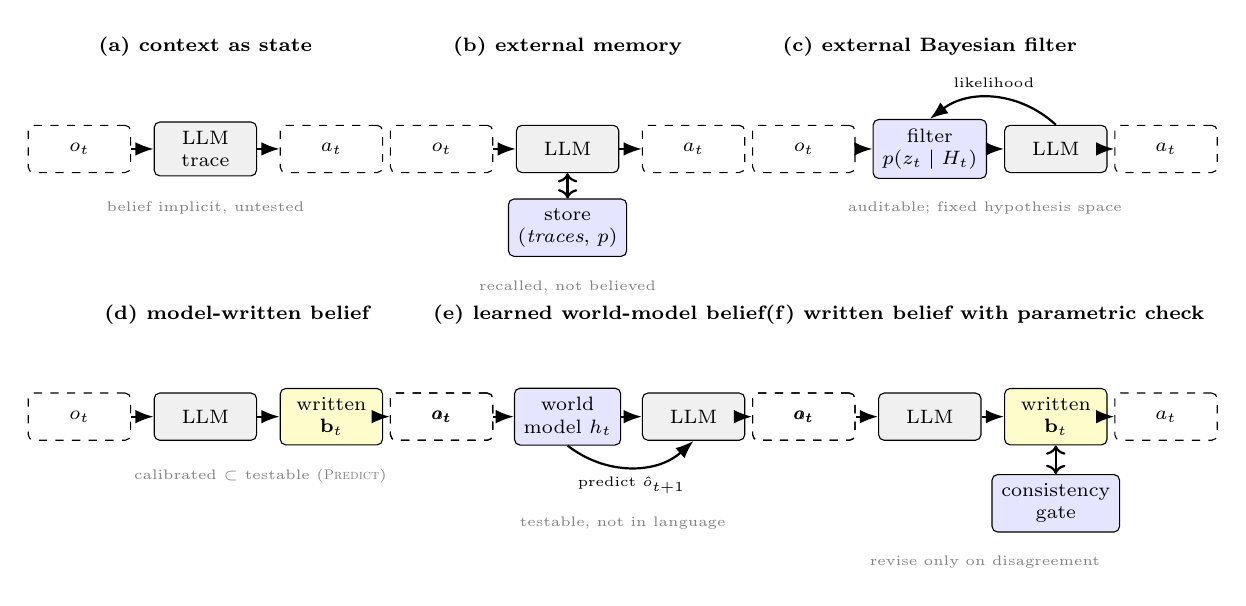
\begin{tikzpicture}[font=\scriptsize,
  llm/.style={draw, rounded corners=2pt, fill=gray!12, minimum width=13mm, minimum height=6mm, align=center},
  bel/.style={draw, rounded corners=2pt, fill=yellow!20, minimum width=13mm, minimum height=6mm, align=center},
  ext/.style={draw, rounded corners=2pt, fill=blue!10, minimum width=13mm, minimum height=6mm, align=center},
  env/.style={draw, dashed, rounded corners=2pt, minimum width=13mm, minimum height=6mm, align=center},
  ttl/.style={font=\scriptsize\bfseries, align=center},
  arr/.style={-{Latex}, thick}]
% panel 1: context as state
\begin{scope}[shift={(0,0)}]
\node[ttl] at (0,1.3) {(a) context as state};
\node[env] (o) at (-1.6,0) {$o_t$};
\node[llm] (m) at (0,0) {LLM\\trace};
\node[env] (a) at (1.6,0) {$a_t$};
\draw[arr] (o)--(m); \draw[arr] (m)--(a);
\node[font=\tiny, text=gray] at (0,-0.75) {belief implicit, untested};
\end{scope}
% panel 2: external / probabilistic memory
\begin{scope}[shift={(4.6,0)}]
\node[ttl] at (0,1.3) {(b) external memory};
\node[env] (o) at (-1.6,0) {$o_t$};
\node[llm] (m) at (0,0) {LLM};
\node[env] (a) at (1.6,0) {$a_t$};
\node[ext] (s) at (0,-1.0) {store\\(\emph{traces}, $p$)};
\draw[arr] (o)--(m); \draw[arr] (m)--(a); \draw[arr,<->] (m)--(s);
\node[font=\tiny, text=gray] at (0,-1.75) {recalled, not believed};
\end{scope}
% panel 3: external Bayesian filter
\begin{scope}[shift={(9.2,0)}]
\node[ttl] at (0,1.3) {(c) external Bayesian filter};
\node[env] (o) at (-1.6,0) {$o_t$};
\node[ext] (f) at (0,0) {filter\\$p(z_t\mid H_t)$};
\node[llm] (m) at (1.6,0) {LLM};
\node[env] (a) at (3.0,0) {$a_t$};
\draw[arr] (o)--(f); \draw[arr] (f)--(m); \draw[arr] (m)--(a);
\draw[arr] (m.north) to[bend right=40] node[above, font=\tiny] {likelihood} (f.north);
\node[font=\tiny, text=gray] at (0.7,-0.75) {auditable; fixed hypothesis space};
\end{scope}
% panel 4: model-written
\begin{scope}[shift={(0,-3.4)}]
\node[ttl] at (0.4,1.3) {(d) model-written belief};
\node[env] (o) at (-1.6,0) {$o_t$};
\node[llm] (m) at (0,0) {LLM};
\node[bel] (b) at (1.6,0) {written\\$\belief_t$};
\node[env] (a) at (3.0,0) {$a_t$};
\draw[arr] (o)--(m); \draw[arr] (m)--(b); \draw[arr] (b)--(a);
\node[font=\tiny, text=gray] at (0.7,-0.75) {calibrated $\subset$ testable (\op{Predict})};
\end{scope}
% panel 5: world model
\begin{scope}[shift={(4.6,-3.4)}]
\node[ttl] at (0.4,1.3) {(e) learned world-model belief};
\node[env] (o) at (-1.6,0) {$o_t$};
\node[ext] (w) at (0,0) {world\\model $h_t$};
\node[llm] (m) at (1.6,0) {LLM};
\node[env] (a) at (3.0,0) {$a_t$};
\draw[arr] (o)--(w); \draw[arr] (w)--(m); \draw[arr] (m)--(a);
\draw[arr] (w.south) to[bend right=40] node[below, font=\tiny] {predict $\hat o_{t+1}$} (m.south);
\node[font=\tiny, text=gray] at (0.7,-1.35) {testable, not in language};
\end{scope}
% panel 6: hybrid check
\begin{scope}[shift={(9.2,-3.4)}]
\node[ttl] at (0.7,1.3) {(f) written belief with parametric check};
\node[env] (o) at (-1.6,0) {$o_t$};
\node[llm] (m) at (0,0) {LLM};
\node[bel] (b) at (1.6,0) {written\\$\belief_t$};
\node[env] (a) at (3.0,0) {$a_t$};
\node[ext] (w) at (1.6,-1.1) {consistency\\gate};
\draw[arr] (o)--(m); \draw[arr] (m)--(b); \draw[arr] (b)--(a); \draw[arr,<->] (b)--(w);
\node[font=\tiny, text=gray] at (0.7,-1.85) {revise only on disagreement};
\end{scope}
\end{tikzpicture}}
\caption{Who maintains the belief. Yellow marks a belief the model writes and can reason about; blue marks an external estimator. Only (c), (d)-testable, (e), and (f) commit to a prediction that later evidence can falsify.}
\label{fig:repr}
\end{figure*}


\begin{table*}[t]
\centering\footnotesize
\resizebox{\textwidth}{!}{%
\begin{tabular}{llcccccl}
\toprule
Class & Method & Model-written & Append-only & Uncertainty & \op{Test} & \op{Revise} & Domain \\
\midrule
Context as state & ReAct \citep{yao2023react} & \cmark & \cmark & \xmark & \xmark & \xmark & general \\
External memory & MemGPT \citep{packer2023memgpt} & \xmark & \xmark & \xmark & \xmark & store update & dialogue \\
Probabilistic memory & BeliefMem \citep{liao2026belief} & \xmark & \xmark & prob. & \xmark & noisy-OR & LoCoMo, ALFWorld \\
Probabilistic memory & D-MEM \citep{song2026d} & \xmark & \xmark & RPE & \xmark & gated write & LoCoMo \\
External filter & Belief-State Engine \citep{chattopadhayay2026belief} & \xmark & \xmark & posterior & \cmark & Bayes & Tiger, security \\
External filter & Belief at Risk \citep{dixon2026belief} & \xmark & \xmark & posterior & \cmark & Bayes & equities \\
Model-written & Agent-BRACE \citep{singh2026agent} & \cmark & \xmark & ordinal & \xmark & RL & ALFWorld-style \\
Model-written & Linguistic forecaster \citep{murphy2026agentic} & \cmark & \cmark & numeric & \cmark & sequential & ForecastBench \\
Model-written & BOND \citep{cui2026distilling} & \cmark & \cmark & posterior tag & \xmark & distilled & negotiation \\
Model-written & CBM \citep{xu2026should} & \cmark & \cmark & \xmark & \cmark (symbolic) & RL & closed world \\
Model-written & EvoSCM \citep{zhao2026evoscm} & \cmark & \cmark & population & \cmark (interventions) & rule distillation & science \\
World model & BB-WM \citep{kumar2026towards} & \xmark & \xmark & latent & \cmark & learned & general \\
\bottomrule
\end{tabular}}
\caption{Belief representation by who maintains the belief. \op{Test}: the belief commits to a falsifiable prediction. All 2026 entries are arXiv preprints at the time of writing; ReAct and MemGPT are peer-reviewed.}
\label{tab:representation}
\end{table*}

\begin{table*}[t]
\centering\footnotesize
\resizebox{\textwidth}{!}{%
\begin{tabular}{lcccccl}
\toprule
Method & Failed stay & Failed update & Failed isolation & Failed act & Trigger & Signal projected to \\
\midrule
Reflexion \citep{shinn2023reflexion} & & \cmark & & & task failure & whole context \\
BeliefShift \citep{myakala2026beliefshift} & \cmark & \cmark & & & user evidence & (benchmark) \\
STALE \citep{chao2026stale} & & \cmark & & \cmark & implicit conflict & (benchmark) \\
CBM \citep{xu2026should} & \cmark & \cmark & \cmark & & symbolic check & belief state \\
TOKI \citep{wang2026toki} & & \cmark & & & contradiction & memory rows \\
MemOps \citep{hao2026memops} & & \cmark & \cmark & & lifecycle op & (benchmark) \\
D-MEM \citep{song2026d} & & \cmark & \cmark & & reward pred. error & memory path \\
STOCKTAKE \citep{deb2026stocktake} & & \cmark & & \cmark & oracle mismatch & (benchmark) \\
Agent-BRACE \citep{singh2026agent} & & \cmark & & \cmark & certainty & belief model \\
Werewolf audit \citep{gao2026auditing} & & \cmark & & \cmark & external belief log & (benchmark) \\
\bottomrule
\end{tabular}}
\caption{Belief revision methods and benchmarks by failure mode addressed, revision trigger, and where the signal is projected.}
\label{tab:revision}
\end{table*}


\begin{table*}[t]
\centering\footnotesize
\resizebox{\textwidth}{!}{%
\begin{tabular}{lllllccc}
\toprule
Level & Representative methods & Feedback source & Granularity & Signed by returned $o_{t+1}$ & Delayed evidence & Partial obs. & Evidence \\
\midrule
Output & SFT, RLHF, DPO \citep{ouyang2022training,rafailov2023direct} & demos, preferences & response & \xmark & \xmark & \xmark & P \\
Trajectory & PPO, GRPO, PRMs \citep{schulman2017proximal,shao2024deepseekmath,lightman2023lets} & verifier, PRM & step / rollout & \xmark & \xmark & \xmark & P \\
Interaction & HiPER, G$^2$PO, ECPO, IAPO \citep{peng2026hiper,wang2026groupgraph,li2026denser,ren2026iapo} & environment & turn / action & \xmark & partial & \xmark & A \\
Interaction & Memory-R2, TAMTRL, EvoHarness-RL \citep{yan2026memoryr2,wang2026tamtrl,ning2026evoharness} & environment, teacher & memory operation & \xmark & partial & \cmark & A \\
State & CBM \citep{xu2026should} & symbolic belief reward & belief state & closed world & \cmark & \cmark & A \\
State & Agent-BRACE \citep{singh2026agent} & joint RL, calibration & claim + certainty & calibration target & \cmark & \cmark & A \\
State & BOND \citep{cui2026distilling} & Bayesian teacher & posterior tag & teacher & \xmark & \cmark & A \\
\bottomrule
\end{tabular}}
\caption{Learning signals by credited object. Evidence: P = peer-reviewed venue, A = arXiv preprint at the time of writing.}
\label{tab:learning}
\end{table*}


\begin{table*}[t]
\centering\footnotesize
\resizebox{\textwidth}{!}{%
\begin{tabular}{llllccl}
\toprule
Benchmark & Domain & Horizon & Latent state & Observable to evaluator & Delayed evidence & Belief-level quantity reported \\
\midrule
ALFWorld \citep{shridhar2020alfworld} & text + embodied & episodic & household state & \cmark & partial & none (task success) \\
PlanBench \citep{valmeekam2022planbench} & classical planning & plan-length & PDDL state & \cmark & \xmark & plan verification, replanning \\
AgentBench \citep{liu2023agentbench} & 8 environments & episodic & environment state & \cmark & partial & none (task success) \\
SmartPlay \citep{wu2023smartplay} & 6 games & episodic & game state & \cmark & partial & none (9 capability scores) \\
T4D / FaR \citep{zhou2023how} & theory of mind & single-turn & others' beliefs & \cmark (annotated) & \xmark & belief tracking vs.\ action selection \\
False-belief tasks \citep{kosinski2023evaluating} & theory of mind & single-turn & others' beliefs & \cmark (annotated) & \xmark & false-belief accuracy \\
LoCoMo \citep{maharana2024evaluating} & long conversations & 35 sessions & conversation facts & annotated & \cmark & temporal QA (proxy) \\
$\tau$-bench / $\tau^2$-bench \citep{yao2024taubench,barres2025tau2bench} & tool--user interaction & multi-turn & database state & \cmark & \cmark & pass\textasciicircum{}k consistency; reasoning vs.\ communication errors \\
MemoryAgentBench \citep{hu2025evaluating} & incremental multi-turn & long-horizon & memory contents & annotated & \cmark & retrieval, test-time learning, conflict resolution \\
BeliefTrack \citep{xu2026should} & closed-world reasoning & multi-turn & finite belief space & \cmark (symbolic) & \cmark & turn-level belief accuracy; failed stay/update/isolation \\
DeltaLogic \citep{dhanda2026deltalogic} & logical reasoning & 2 steps & premise set & \cmark & \cmark & revision accuracy vs.\ initial accuracy \\
DToM-Track \citep{nguyen2026dynamic} & dialogue & multi-turn & interlocutor belief & \cmark (annotated) & \cmark & prior-belief recall; change detection \\
BeliefShift \citep{myakala2026beliefshift} & user modelling & multi-session & user opinion & annotated & \cmark & revision accuracy; drift coherence; evidence sensitivity \\
OmniToM \citep{bawatneh2026omnitom} & theory of mind & narrative & actors' beliefs & \cmark (annotated) & \xmark & belief-proposition extraction; schema labels \\
MINDGAMES \citep{wang2026mindgames} & social games & repeated games & hidden roles, opponents & \cmark & \cmark & TrueSkill; turn-level logs \\
MEDLEY-BENCH \citep{abtahi2026medleybench} & social pressure & 2 rounds & --- & \xmark & \xmark & sensitivity to manipulated consensus \\
STALE \citep{chao2026stale} & memory validity & multi-turn & fact validity & annotated & \cmark & state resolution; premise resistance; policy adaptation \\
MemOps \citep{hao2026memops} & long conversations & multi-session & memory lifecycle & annotated & \cmark & operation-level probes \\
GroupMemBench \citep{yang2026groupmembench} & multi-party dialogue & multi-session & per-speaker knowledge & annotated & \cmark & information-update accuracy \\
MemGym \citep{xu2026memgym} & mixed agent tasks & long-horizon & --- & \xmark & partial & memory-isolated score delta \\
STOCKTAKE \citep{deb2026stocktake} & inventory control & weekly, long & demand factors & \cmark (Bayes filter) & \cmark & detection lag; skill vs.\ oracle; knowing-doing rate \\
Flux \citep{alaswad2026why} & text game & long-horizon & simulator state & \cmark & \cmark & state-tracking error modes \\
YC-Bench \citep{he2026ycbench} & startup simulation & hundreds of turns & market, clients & privileged outcome & \cmark & scratchpad usage (proxy) \\
RetailBench \citep{zhang2026retailbenchx} & retail POMDP & 180 days & demand, supply & privileged oracle & \cmark & evidence-acquisition behaviour (proxy) \\
EnterpriseArena \citep{han2026can} & lending & 132 months & borrower pool & privileged outcome & \cmark & observation-budget allocation (proxy) \\
Business Arena \citep{pan2026business} & marketplace & long-horizon & market & privileged outcome & \cmark & action-level attribution \\
Werewolf audit \citep{gao2026auditing} & social deduction & 9-player game & roles & \cmark & \cmark & action--belief consistency \\
CAGE-2 study \citep{bogdanov2026context} & cyber defence & episodic & network state & \cmark & partial & state-abstraction return gain \\
MD5 state tracking \citep{pai2026longhorizon} & tool chains & 196 calls & registers & \cmark & \xmark & exact-state success \\
FinBench (time-gated) \citep{ghosh2026finbench} & asset forecasting & daily & returns & realised & \cmark & Brier; interval scores \\
TradeArena \citep{xue2026representation} & trading & multi-week & regimes & realised & \cmark & representation drift (early warning) \\
HERCULEAN \citep{herculean2026} & finance workflows & multi-step & market, books & partial & \cmark & state-tracking sub-score \\
FinBen / InvestorBench \citep{xie2025finben,li2024investorbench} & finance tasks / trading & task / episodic & --- & \xmark & partial & none (outcome only) \\
\bottomrule
\end{tabular}}
\caption{Benchmarks that exercise belief maintenance, by whether the evaluator can observe the latent state and what belief-level quantity is reported. \lq\lq{}Annotated\rq\rq{} means human labels stand in for the latent state; \lq\lq{}privileged\rq\rq{} means the simulator knows it but the benchmark reports only outcomes. Ev.\ column omitted for space; peer-reviewed entries are ALFWorld, PlanBench, AgentBench, SmartPlay, T4D, false-belief tasks, LoCoMo, FinBen, and InvestorBench; the rest are arXiv preprints at the time of writing.}
\label{tab:benchmarks}
\end{table*}


\begin{table*}[t]
\centering\tiny
\setlength{\tabcolsep}{2.5pt}
\resizebox{\textwidth}{!}{%
\begin{tabular}{lcllllc}
\toprule
System & Year & Belief kept by & Credited & Revision trigger & Metric & Ev. \\
\midrule
Schema-driven DST \citep{lee2021dialogue} & 2021 & written & none & dialogue history plus schema\ldots & \cmark & P \\
Verbalized Uncertainty \citep{lin2022teaching} & 2022 & written & output & fine-tuning on calibrated\ldots & \cmark & P \\
LMs Know \citep{kadavath2022language} & 2022 & written & output & self-evaluation P and P of\ldots & \cmark & A \\
DreamerV3 \citep{hafner2023mastering} & 2023 & world model & world-model loss & RSSM latent posterior updated\ldots & $\circ$ & P \\
RecurrentGPT \citep{zhou2023recurrentgpt} & 2023 & written & output & LLM rewrites its own\ldots &  & A \\
LLM-MCTS \citep{zhao2023large} & 2023 & world model & trajectory & LLM-sampled world state\ldots & $\circ$ & P \\
RAP \citep{hao2023reasoning} & 2023 & world model & trajectory & LLM-as-world-model predicted\ldots &  & P \\
Reflect-RL \citep{zhou2024reflectrl} & 2024 & written & interaction & frozen reflection model\ldots &  & P \\
Hypothetical Minds \citep{cross2024hypothetical} & 2024 & written & none & hypotheses about other\ldots & $\circ$ & A \\
Talker-Reasoner \citep{christakopoulou2024agents} & 2024 & written & none & Reasoner writes/updates\ldots &  & A \\
QuBE \citep{kim2024qube} & 2024 & written & none & question-answering over\ldots &  & P \\
MEM1 \citep{zhou2025mem1} & 2025 & written & outcome (written state) & internal state rewritten each\ldots & $\circ$ & A \\
MemAgent \citep{yu2025memagent} & 2025 & written & outcome (written state) & chunk-wise overwrite of\ldots & $\circ$ & P \\
PCE \citep{seo2026assumptions} & 2026 & written & none & scenario likelihood scoring & $\circ$ & A \\
RB-VLA \citep{bagaria2026recursive} & 2026 & world model & world-model loss & self-supervised world-model\ldots & $\circ$ & A \\
REDEREF \citep{hosseini2026trainingfree} & 2026 & prob.\ memory & interaction & judge feedback updates\ldots &  & A \\
TAMTRL \citep{wang2026tamtrl} & 2026 & written & trajectory & teacher likelihood of memory\ldots & $\circ$ & A \\
Self-Guide internal\ldots \citep{wang2026coevolution} & 2026 & written & trajectory & self-generated guidance as\ldots &  & A \\
ReflectiChain\ldots \citep{luo2026topology} & 2026 & world model & trajectory & latent trajectory rehearsal\ldots &  & A \\
\bottomrule
\end{tabular}\hfill
\begin{tabular}{lcllllc}
\toprule
System & Year & Belief kept by & Credited & Revision trigger & Metric & Ev. \\
\midrule
Cyclic subtask graphs \citep{gharzeddine2026complete} & 2026 & written & none & state-analysis-and-routing\ldots &  & A \\
CHAL \citep{giovannelli2026chal} & 2026 & written & none & gradient-informed revision on\ldots & $\circ$ & A \\
Pinductor \citep{six2026learning} & 2026 & world model & world-model loss & belief-based likelihood score\ldots & $\circ$ & A \\
Belief Engine stance\ldots \citep{yang2026belief} & 2026 & prob.\ memory & none & log-odds update with evidence\ldots & \cmark & A \\
HIPIF \citep{diao2026hipif} & 2026 & written & trajectory & subgoal completion +\ldots &  & A \\
ProPlay \citep{ma2026proplay} & 2026 & world model & trajectory & post-episode graph refinement\ldots & $\circ$ & A \\
POMDP validation\ldots \citep{dixon2026model} & 2026 & ext.\ filter & none & Bayesian & \cmark & A \\
Internalizing the Future \citep{zhang2026internalizing} & 2026 & written & trajectory & foresight-conditioned RL\ldots & $\circ$ & A \\
Hybrid-WM \citep{song2026agent} & 2026 & world model & world-model loss & consistency gate & \cmark & A \\
Governance-aware POMDP\ldots \citep{dixon2026adaptive} & 2026 & ext.\ filter & none & Bayesian update on evidence\ldots & $\circ$ & A \\
BayesEvolve \citep{wu2026bayesevolve} & 2026 & ext.\ filter & none & posterior refit after each\ldots & \cmark & A \\
WorldEvolver \citep{zhang2026selfevolvingx} & 2026 & world model & world-model loss & prediction-observation\ldots & $\circ$ & A \\
WM-SAR \citep{song2026repair} & 2026 & world model & trajectory & spectral error amplification &  & A \\
BCO \citep{chen2026beliefcalibrated} & 2026 & written & none & evaluation of new candidate\ldots & \cmark & A \\
EvoSCM causal belief\ldots \citep{zhao2026evoscm} & 2026 & written & none & prediction-observation\ldots & \cmark & A \\
CAPTURE \citep{hossain2026capture} & 2026 & world model & world-model loss & uncertainty-triggered\ldots & \cmark & A \\
Semantic Bayesian World\ldots \citep{soru2026semantic} & 2026 & ext.\ filter & none & Bayesian conditioning on\ldots &  & A \\
Belief-State Engine \citep{chattopadhayay2026belief} & 2026 & ext.\ filter & none (prompting) & Bayesian posterior & \cmark & A \\
\bottomrule
\end{tabular}}
\caption{Systems with an explicit belief mechanism, by year. Belief kept by: who maintains the belief (Section~\ref{sec:representation}); Credited: the object that receives the learning signal under the criterion of Section~\ref{sec:learning}, \emph{none} if the belief is not trained; Metric: \cmark\ reports a belief-level quantity, $\circ$ a proxy; Ev.: P peer-reviewed, A arXiv preprint.}
\label{tab:master}
\end{table*}


\begin{table*}[t]
\centering\tiny
\setlength{\tabcolsep}{2.5pt}
\resizebox{\textwidth}{!}{%
\begin{tabular}{lcllllc}
\toprule
System & Year & Belief kept by & Credited & Revision trigger & Metric & Ev. \\
\midrule
Decision Transformer \citep{chen2021decision} & 2021 & context & interaction & return-to-go conditioning\ldots &  & P \\
Schema-driven DST \citep{lee2021dialogue} & 2021 & written & none & dialogue history plus schema\ldots & \cmark & P \\
Chain-of-Thought \citep{wei2022chain} & 2022 & context & output & none &  & P \\
Verbalized Uncertainty \citep{lin2022teaching} & 2022 & written & output & fine-tuning on calibrated\ldots & \cmark & P \\
LMs Know \citep{kadavath2022language} & 2022 & written & output & self-evaluation P and P of\ldots & \cmark & A \\
Inner Monologue \citep{huang2022inner} & 2022 & context & interaction & success detection, scene\ldots &  & P \\
DreamerV3 \citep{hafner2023mastering} & 2023 & world model & world-model loss & RSSM latent posterior updated\ldots & $\circ$ & P \\
DEPS \citep{wang2023describe} & 2023 & context & trajectory & descriptor of execution\ldots &  & P \\
Reflexion \citep{shinn2023reflexion} & 2023 & ext.\ memory & trajectory & verbal self-reflection after\ldots &  & P \\
RCI \citep{kim2023language} & 2023 & context & interaction & recursive self-criticism of\ldots &  & P \\
Self-Refine \citep{madaan2023self} & 2023 & context & output & self-generated\ldots &  & P \\
Generative Agents \citep{park2023generative} & 2023 & ext.\ memory & interaction & observation stream; periodic\ldots &  & P \\
Self-Debug \citep{chen2023teaching} & 2023 & context & output & execution feedback +\ldots &  & P \\
Tree of Thoughts \citep{yao2023tree} & 2023 & context & trajectory & self-evaluation of\ldots &  & P \\
MemoryBank \citep{zhong2023memorybank} & 2023 & ext.\ memory & output & Ebbinghaus-style forgetting\ldots &  & P \\
RecurrentGPT \citep{zhou2023recurrentgpt} & 2023 & written & output & LLM rewrites its own\ldots &  & A \\
LLM-MCTS \citep{zhao2023large} & 2023 & world model & trajectory & LLM-sampled world state\ldots & $\circ$ & P \\
RAP \citep{hao2023reasoning} & 2023 & world model & trajectory & LLM-as-world-model predicted\ldots &  & P \\
Voyager \citep{wang2023voyager} & 2023 & ext.\ memory & trajectory & environment execution\ldots &  & P \\
ExpeL \citep{zhao2023expel} & 2023 & ext.\ memory & trajectory & cross-task insight extraction\ldots &  & P \\
CoALA \citep{sumers2023cognitive} & 2023 & ext.\ memory & none & conceptual &  & P \\
TradingGPT \citep{li2023tradinggpt} & 2023 & ext.\ memory & interaction & layered memory decay +\ldots &  & A \\
FaR / T4D \citep{zhou2023how} & 2023 & context & interaction & foresee-and-reflect\ldots & $\circ$ & P \\
LATS \citep{zhou2023language} & 2023 & ext.\ memory & trajectory & MCTS backup of LM-valued\ldots & $\circ$ & P \\
FireAct \citep{chen2023fireact} & 2023 & context & trajectory & supervised fine-tuning on\ldots &  & A \\
MemGPT \citep{packer2023memgpt} & 2023 & ext.\ memory & output & self-directed memory paging\ldots &  & A \\
AgentTuning \citep{zeng2023agenttuning} & 2023 & context & trajectory & hybrid instruction tuning on\ldots &  & P \\
FinMem \citep{yu2023finmem} & 2023 & ext.\ memory & interaction & layered memory with\ldots &  & P \\
Reflect-RL \citep{zhou2024reflectrl} & 2024 & written & interaction & frozen reflection model\ldots &  & P \\
FinAgent \citep{zhang2024multimodal} & 2024 & ext.\ memory & interaction & low-level and high-level\ldots &  & P \\
AgentGym \citep{xi2024agentgym} & 2024 & context & trajectory & AgentEvol &  & A \\
Hypothetical Minds \citep{cross2024hypothetical} & 2024 & written & none & hypotheses about other\ldots & $\circ$ & A \\
FinCon \citep{yu2024fincon} & 2024 & ext.\ memory & none & episodic self-critique\ldots &  & P \\
Agent Q \citep{putta2024agent} & 2024 & ext.\ memory & trajectory & MCTS with AI self-critique\ldots & $\circ$ & A \\
Agent Workflow Memory \citep{wang2024agent} & 2024 & ext.\ memory & none & induction of reusable\ldots &  & A \\
Talker-Reasoner \citep{christakopoulou2024agents} & 2024 & written & none & Reasoner writes/updates\ldots &  & A \\
QuBE \citep{kim2024qube} & 2024 & written & none & question-answering over\ldots &  & P \\
TradingAgents \citep{xiao2024tradingagents} & 2024 & context & output & multi-agent debate and\ldots &  & A \\
AgentRefine \citep{fu2025agentrefine} & 2025 & context & trajectory & environment observation\ldots &  & P \\
LOOP \citep{chen2025reinforcement} & 2025 & context & trajectory & environment feedback via API\ldots &  & A \\
A-Mem \citep{xu2025mem} & 2025 & ext.\ memory & output & memory evolution &  & P \\
Search-R1 \citep{jin2025searchr1} & 2025 & context & output & retrieved documents\ldots &  & A \\
ReSearch \citep{chen2025research} & 2025 & context & output & search results inserted into\ldots &  & P \\
RAGEN / StarPO \citep{wang2025ragen} & 2025 & context & trajectory & environment reward\ldots &  & A \\
Mem0 \citep{chhikara2025mem0} & 2025 & ext.\ memory & none & LLM-driven extraction\ldots &  & A \\
TTI \citep{shen2025thinking} & 2025 & context & trajectory & additional environment\ldots &  & A \\
MEM1 \citep{zhou2025mem1} & 2025 & written & outcome (written state) & internal state rewritten each\ldots & $\circ$ & A \\
MemAgent \citep{yu2025memagent} & 2025 & written & outcome (written state) & chunk-wise overwrite of\ldots & $\circ$ & P \\
ARPO \citep{dong2025agentic} & 2025 & context & trajectory & token entropy spike after\ldots & $\circ$ & A \\
Memento \citep{zhou2025memento} & 2025 & ext.\ memory & interaction & environment feedback rewrites\ldots &  & A \\
Agent-R1 \citep{cheng2025agentr1} & 2025 & context & trajectory & tool/environment feedback per\ldots &  & A \\
MATTRL test-time\ldots \citep{hu2026collaborative} & 2026 & ext.\ memory & interaction & turn-level credit for\ldots &  & A \\
SuS strategy-aware\ldots \citep{kashirskiy2026sus} & 2026 & context & output & surprise residual &  & A \\
External affective\ldots \citep{subaharan2026controlling} & 2026 & ext.\ memory & none & exponential smoothing or\ldots &  & A \\
PCE \citep{seo2026assumptions} & 2026 & written & none & scenario likelihood scoring & $\circ$ & A \\
HiPER \citep{peng2026hiper} & 2026 & context & trajectory & none &  & A \\
RB-VLA \citep{bagaria2026recursive} & 2026 & world model & world-model loss & self-supervised world-model\ldots & $\circ$ & A \\
REDEREF \citep{hosseini2026trainingfree} & 2026 & prob.\ memory & interaction & judge feedback updates\ldots &  & A \\
DenoiseFlow \citep{yan2026denoiseflow} & 2026 & context & trajectory & semantic entropy over samples & $\circ$ & A \\
MICA \citep{zhang2026mica} & 2026 & ext.\ memory & interaction & none &  & A \\
\bottomrule
\end{tabular}\hfill
\begin{tabular}{lcllllc}
\toprule
System & Year & Belief kept by & Credited & Revision trigger & Metric & Ev. \\
\midrule
HCAPO hindsight critic \citep{tan2026hindsight} & 2026 & context & trajectory & post-hoc LLM critic refinement &  & A \\
TIPS \citep{xie2026tips} & 2026 & context & interaction & teacher answer-likelihood gain & $\circ$ & A \\
DToM-Track \citep{nguyen2026dynamic} & 2026 & context & none & none & \cmark & A \\
D-MEM \citep{song2026d} & 2026 & ext.\ memory & none & reward prediction error gating & $\circ$ & A \\
SLEA-RL \citep{wang2026slearl} & 2026 & ext.\ memory & trajectory & observation change triggers\ldots &  & A \\
Graph of States \citep{luo2026graph} & 2026 & ext.\ memory & none & symbolic check &  & A \\
TAMTRL \citep{wang2026tamtrl} & 2026 & written & trajectory & teacher likelihood of memory\ldots & $\circ$ & A \\
MT-GRPO Iterative\ldots \citep{modecrua2026multiturn} & 2026 & context & interaction & none &  & A \\
Self-Guide internal\ldots \citep{wang2026coevolution} & 2026 & written & trajectory & self-generated guidance as\ldots &  & A \\
SAVeR \citep{yuan2026verify} & 2026 & context & none & adversarial audit locating\ldots & $\circ$ & A \\
ReflectiChain\ldots \citep{luo2026topology} & 2026 & world model & trajectory & latent trajectory rehearsal\ldots &  & A \\
Cyclic subtask graphs \citep{gharzeddine2026complete} & 2026 & written & none & state-analysis-and-routing\ldots &  & A \\
CAPO \citep{wang2026capo} & 2026 & context & interaction & none &  & A \\
AEM adaptive entropy\ldots \citep{zhao2026aem} & 2026 & context & trajectory & response-level surprisal x\ldots &  & A \\
T2PO \citep{wang2026t2po} & 2026 & context & interaction & token-level\ldots & $\circ$ & A \\
MedExAgent \citep{gao2026medexagent} & 2026 & context & output & none &  & A \\
TRACE turn credit for\ldots \citep{he2026turns} & 2026 & context & interaction & leave-one-turn-out semantic\ldots &  & A \\
PiCA pivot-based credit \citep{liu2026pica} & 2026 & context & trajectory & pivot-step potential-based\ldots &  & A \\
CHAL \citep{giovannelli2026chal} & 2026 & written & none & gradient-informed revision on\ldots & $\circ$ & A \\
Why world models \citep{alaswad2026why} & 2026 & context & none & none & $\circ$ & A \\
Pinductor \citep{six2026learning} & 2026 & world model & world-model loss & belief-based likelihood score\ldots & $\circ$ & A \\
Belief Engine stance\ldots \citep{yang2026belief} & 2026 & prob.\ memory & none & log-odds update with evidence\ldots & \cmark & A \\
CAGE-2 compound agent\ldots \citep{bogdanov2026context} & 2026 & ext.\ memory & none & deterministic state-tracking\ldots &  & A \\
Representation\ldots \citep{xue2026representation} & 2026 & context & output & structured risk feedback & $\circ$ & A \\
CMI \citep{srivastava2026causal} & 2026 & ext.\ memory & none & counterfactual answer-score\ldots & $\circ$ & A \\
SERL selective\ldots \citep{li2026what} & 2026 & context & interaction & per-step environment feedback\ldots &  & A \\
Memory-R2 / LoGo-GRPO \citep{yan2026memoryr2} & 2026 & ext.\ memory & none & local rerollouts from shared\ldots & $\circ$ & A \\
SkillC \citep{lin2026skillc} & 2026 & context & trajectory & skill-vs-no-skill reward gap &  & A \\
InKH financial harness \citep{borjigin2026absorbing} & 2026 & ext.\ memory & none & passive knowledge injection\ldots & $\circ$ & A \\
TOKI \citep{wang2026toki} & 2026 & ext.\ memory & none & bitemporal operators & $\circ$ & A \\
Q-Evolve \citep{zhang2026selfevolving} & 2026 & context & trajectory & advantage from\ldots &  & A \\
HIPIF \citep{diao2026hipif} & 2026 & written & trajectory & subgoal completion +\ldots &  & A \\
ProPlay \citep{ma2026proplay} & 2026 & world model & trajectory & post-episode graph refinement\ldots & $\circ$ & A \\
POMDP validation\ldots \citep{dixon2026model} & 2026 & ext.\ filter & none & Bayesian & \cmark & A \\
G2PO \citep{wang2026groupgraph} & 2026 & context & trajectory & globally standardized TD\ldots &  & A \\
Internalizing the Future \citep{zhang2026internalizing} & 2026 & written & trajectory & foresight-conditioned RL\ldots & $\circ$ & A \\
Hybrid-WM \citep{song2026agent} & 2026 & world model & world-model loss & consistency gate & \cmark & A \\
Governance-aware POMDP\ldots \citep{dixon2026adaptive} & 2026 & ext.\ filter & none & Bayesian update on evidence\ldots & $\circ$ & A \\
BayesEvolve \citep{wu2026bayesevolve} & 2026 & ext.\ filter & none & posterior refit after each\ldots & \cmark & A \\
WorldEvolver \citep{zhang2026selfevolvingx} & 2026 & world model & world-model loss & prediction-observation\ldots & $\circ$ & A \\
WM-SAR \citep{song2026repair} & 2026 & world model & trajectory & spectral error amplification &  & A \\
STAPO\ldots \citep{qi2026stapo} & 2026 & context & trajectory & normalized-entropy outlier\ldots &  & A \\
Auditing\ldots \citep{gao2026auditing} & 2026 & ext.\ memory & none & logged per-turn belief updates & \cmark & A \\
RLAW \citep{ali2026reward} & 2026 & ext.\ memory & interaction & critique score &  & A \\
NeSyFS \citep{xu2026nesyfs} & 2026 & ext.\ memory & interaction & repeated fast-action failure\ldots &  & A \\
MADE \citep{liu2026made} & 2026 & ext.\ memory & interaction & execution failure ->\ldots &  & A \\
MD5 state tracking \citep{pai2026longhorizon} & 2026 & context & none & majority vote over arithmetic &  & A \\
TCPO turn-level credit \citep{liao2026tcpo} & 2026 & context & interaction & verifier score-to-credit\ldots &  & A \\
When Memory Updates but\ldots \citep{sun2026memory} & 2026 & ext.\ memory & none & stale dependency repair & $\circ$ & A \\
EvoHarness-RL learned\ldots \citep{ning2026evoharness} & 2026 & ext.\ memory & interaction & learned\ldots & $\circ$ & A \\
GPM \citep{xu2026governed} & 2026 & ext.\ memory & none & symbolic check & $\circ$ & A \\
CrEST \citep{wang2026teach} & 2026 & context & interaction & verified turn reward with\ldots &  & A \\
HiDiffTIR \citep{guo2026hidifftir} & 2026 & context & interaction & group tool-call success rate &  & A \\
IAPO \citep{ren2026iapo} & 2026 & context & interaction & none &  & A \\
BCO \citep{chen2026beliefcalibrated} & 2026 & written & none & evaluation of new candidate\ldots & \cmark & A \\
EvoSCM causal belief\ldots \citep{zhao2026evoscm} & 2026 & written & none & prediction-observation\ldots & \cmark & A \\
CAPTURE \citep{hossain2026capture} & 2026 & world model & world-model loss & uncertainty-triggered\ldots & \cmark & A \\
PGPO \citep{zheng2026pgpo} & 2026 & context & interaction & potential difference between\ldots &  & A \\
Semantic Bayesian World\ldots \citep{soru2026semantic} & 2026 & ext.\ filter & none & Bayesian conditioning on\ldots &  & A \\
Belief-State Engine \citep{chattopadhayay2026belief} & 2026 & ext.\ filter & none (prompting) & Bayesian posterior & \cmark & A \\
\bottomrule
\end{tabular}}
\caption{All 120 screened systems with a state or memory mechanism, by year (columns as in Table~\ref{tab:master}).}
\label{tab:master_full}
\end{table*}


\section{Timeline of Credited Objects}
\label{app:taxonomy}

\begin{figure*}[h]
\centering
\resizebox{\textwidth}{!}{%
\begin{tikzpicture}[x=2.0cm, y=0.85cm, font=\scriptsize,
  lane/.style={font=\scriptsize\bfseries, anchor=east},
  pt/.style={circle, fill=gray!60, inner sep=1.4pt},
  ptS/.style={circle, fill=red!70!black, inner sep=1.7pt},
  lbl/.style={font=\tiny, anchor=west, inner sep=1pt},
  lblS/.style={font=\tiny, anchor=west, inner sep=1pt, text=red!60!black}]
\foreach \yr/\x in {2020/0, 2021/1, 2022/2, 2023/3, 2024/4, 2025/5, 2026/6} {
  \node[font=\scriptsize\bfseries] at (\x,0.55) {\yr};
  \draw[gray!30] (\x,0.3) -- (\x,-4.8); }
\fill[yellow!15] (-0.1,-4.75) rectangle (7.2,-3.5);
\foreach \name/\y in {{\textbf{output}: response credited}/-1, {\textbf{trajectory}: steps credited}/-2, {\textbf{interaction}: actions, memory ops}/-3, {\textbf{state}: written belief}/-4}
  \node[lane] at (-0.15,\y) {\name};
\foreach \y in {-1,-2,-3,-4} \draw[gray!50] (-0.1,\y) -- (7.2,\y);
% output lane
\node[pt] at (2.1,-1) {}; \node[lbl] at (2.15,-0.74) {CoT, InstructGPT};
\node[pt] at (2.6,-1) {}; \node[lbl] at (2.65,-1.26) {Self-Consistency};
\node[pt] at (3.3,-1) {}; \node[lbl] at (3.35,-0.74) {Self-Refine, Self-Debug};
\node[pt] at (3.95,-1) {}; \node[lbl] at (4.0,-1.26) {MemGPT, MemoryBank};
\node[pt] at (5.2,-1) {}; \node[lbl] at (5.25,-0.74) {A-MEM, Mem0, Search-R1};
% trajectory lane
\node[pt] at (1.5,-2) {}; \node[lbl] at (1.55,-1.74) {Decision Transformer};
\node[pt] at (3.1,-2) {}; \node[lbl] at (3.15,-2.26) {ReAct, Reflexion, RAP, ToT};
\node[pt] at (3.75,-2) {}; \node[lbl] at (3.8,-1.74) {LATS, ExpeL, AgentTuning};
\node[pt] at (4.5,-2) {}; \node[lbl] at (4.55,-2.26) {PRMs, GRPO, Agent Q};
\node[pt] at (5.4,-2) {}; \node[lbl] at (5.45,-1.74) {RAGEN, GiGPO, AgentRefine};
% interaction lane
\node[pt] at (2.3,-3) {}; \node[lbl] at (2.35,-2.74) {SayCan, Inner Monologue};
\node[pt] at (3.2,-3) {}; \node[lbl] at (3.25,-3.26) {Voyager, Generative Agents};
\node[pt] at (4.1,-3) {}; \node[lbl] at (4.15,-2.74) {ArCHer, WebRL, FinAgent};
\node[pt] at (5.1,-3) {}; \node[lbl] at (5.15,-3.26) {LOOP, SWEET-RL, ARPO, Memento};
\node[pt] at (6.1,-3) {}; \node[lbl] at (6.15,-2.74) {HiPER, G$^2$PO, Memory-R2};
% state lane (three label rows)
\node[pt] at (1.6,-4) {}; \node[lbl] at (1.65,-3.72) {schema-driven DST};
\node[pt] at (2.5,-4) {}; \node[lbl] at (2.55,-4.26) {verbalised uncertainty};
\node[pt] at (3.7,-4) {}; \node[lbl] at (3.75,-3.72) {CoALA (framing)};
\node[pt] at (4.35,-4) {}; \node[lbl] at (4.4,-4.26) {QuBE, Talker-Reasoner};
\node[pt] at (4.6,-4) {}; \node[lbl] at (4.5,-4.56) {Hypothetical Minds, FinCon};
\node[pt] at (5.4,-4) {}; \node[lbl] at (5.45,-3.72) {MEM1, MemAgent};
\node[ptS] at (5.85,-4) {}; \node[lblS] at (5.9,-4.26) {Belief-State Engine, Agent-BRACE, BOND, CBM};
\node[ptS] at (6.3,-4) {}; \node[lblS] at (6.35,-3.72) {EvoSCM, BCO, BB-WM};
% legend
\node[draw, rounded corners=2pt, fill=blue!6, align=left, font=\tiny, anchor=north west, inner sep=3pt, text width=16.2cm] at (-3.2,-5.0) {%
\textbf{Axes of the taxonomy.}\quad
\S\ref{sec:representation} who maintains the belief: context $\cdot$ external memory $\cdot$ probabilistic memory $\cdot$ external filter $\cdot$ written $\cdot$ world model.\quad
\S\ref{sec:revision} failure mode: stay $\cdot$ update $\cdot$ isolation $\cdot$ act.\quad
\S\ref{sec:learning} credited object: one lane each.\quad
{\color{red!60!black}$\bullet$} belief trained against evidence (2026).};
\end{tikzpicture}}
\caption{Where credit has gone, 2020--2026. Lanes are credited objects; Table~\ref{tab:master} lists every screened system. Written beliefs exist from dialogue state tracking onward, but until 2026 they are credited by task outcome or not trained at all; the red points are the first to give the belief its own learning signal.}
\label{fig:timeline}
\end{figure*}



\end{document}
